\chapter{The System of Linear Transformations}
\label{chapter-linear-systems}
From now on, we concentrate on the systems of linear transformations between vector spaces over the field $\mathbb{Z}_2$. The reason is simple, they allow a construction of a remarkable model of universal hashing. Like for the other universal models, the expected length of a chain is constant and so is the expected running time of the find operation. In addition, the expected length of the longest chain is bounded by a sub-linear function of a single variable -- the size of the hash table. In our model, we have also managed to prove that the expected amortised time of every operation, find, insert and delete, is constant.

Once again, the main result is the upper bound on the expected length of the longest chain when a system of linear maps is used as a universal class. As already mentioned, probability of collision of $k$-elements is not estimated directly from the properties common to all universal systems. Hence the proof of the bound can not be based on the idea shown in the previous chapter.

First, we show a few models of the uniform random choice of a linear function. They describe other ways of the uniform random choice of a linear function from the universal class -- choice of the universal hash function. Later, we prove some technical lemmas regarding the vector spaces. Finally, we state the required facts in terms of system of linear transformations. Then we interpret the facts in terms of hashing and propose a new model. Many theorems come from \cite{DBLP:journals/jacm/AlonDMPT99}. Our work lies in their correction, improvement and modification leading to a better and practical result.

In the following sections we restrict ourselves only to the vector spaces over the field $\mathbb{Z}_2$. If vector spaces are taken over other finite field than the field $\mathbb{Z}_2$, then we can not expect such good results as shown in \cite{DBLP:journals/jacm/AlonDMPT99}. The original result proposes hashing of $m \log m$ elements into a hash table of size of $m$ slots and leads to the bound $O(\log m \log \log m)$. Although the result may already be used for hashing $m$ elements, too, it is later improved for $\alpha \leq 1$.

When unsure about any exact definition or fact from linear algebra, see Appendix~\ref{appendix-linear-algebra} where we exactly summarise and accurately state them.

\begin{section}{Models of uniform choice of a linear map}
Technical preparations also include some models which show how uniform choice of a random linear map can be performed. These models are later used to simplify some proofs assuming uniform choice of linear transformation. Instead of simply choosing linear map we select other objects that uniquely define a linear function and work with them. When uniformly performing mentioned selections we obtain uniform selection of suitable linear function.

Definition $\ref{definition-system-of-linear-transformations}$ of systems of linear maps can be extended to denote not only the sets of all linear maps but all surjective linear maps as well. This notation is especially useful when considering various models of choice of (surjective) linear transformation.
\begin{definition}
Let $A$ and $B$ be two vector spaces. Define the set of all linear transformations
\[
LT(A, B) = \{ T: A \rightarrow B \setdelim T \text{ linear transformation} \}
\]
and
\[
LTS(A, B) = \{ T: A \rightarrow B \setdelim T \text{ surjective linear transformation} \}
\] set of all surjective linear transformations between vector spaces $A$ and $B$.
\end{definition} 

\begin{definition}[Uniform selection model]
Let $A$ be a set such that $A = \{ a_1, \dots, a_n \}$. By random uniform selection of element $a \in A$ we understand a model of selection where 
\[
	\Prob{a \in A \text{ was selected}} = \frac{1}{n} \text{.}
\]
\end{definition}

The first model depicts correspondence between uniform choice of a basis of the source space that is mapped onto a fixed basis of the target space and uniform choice of surjective linear transformation.
\begin{remark}[Surjective linear map selection]
\label{remark-model-surjective-linear-map-selection}
Let $\mathcal{B}$ be a set of all bases of vector space $\mathbb{Z}_2^u$ and $\{y_1, \dots, y_t\}$ be a basis of vector space $\mathbb{Z}_2^t$ where $t \leq u$ and let vectors in bases be lexicographically ordered. Define \[\mathcal{S} = \{\{a_1, \dots, a_{u - t}\} \setdelim 1 \leq a_1 < \dots < a_{u-t} \leq u \} \text{.} \] For a random uniform choice of basis $b = \{b_1, \dots, b_u\} \in \mathcal{B}$, $s \in \mathcal{S}$ and permutation $\pi \in \Pi_t$ define linear map $T_{b, s, \pi}$ as
\[
T_{b, s, \pi}(b_i) =  
  \begin{cases} 
    y_{\pi(i)} & \text{if } i \notin s \\
    0 & \text{if } i \in s
  \end{cases} \text{.}
\]
If we perform these random uniform choices of $b, s$ and $\pi$ we obtain randomly and uniformly selected surjective linear map $T_{b, s, \pi}$.
\end{remark}
\begin{proof}
First remark that $T_{b, s, \pi}$ is a surjective linear map for every choice of $b \in \mathcal{B}$ and $s \in \mathcal{S}$. From the fact that $T_{b, s, \pi}$ is defined for every vector of the basis $b$ we known it may be uniquely extended to a linear map. It is surjective since for every vector $y_i$, $1 \leq i \leq t$ there is a vector $b_j$, $1 \leq j \leq u$ such that $T_{b, s, \pi}(b_j) = y_i$. 

Now we show that for every surjective linear transformation $T$ there is a choice $b, s$ and $\pi$ such that $T_{b, s, \pi} = T$. Consider set $T^{-1}(0)$, it certainly contains $t$ linearly independent vectors, denote them as $B_0$. Now consider set $\mathbb{Z}_2^u - T^{-1}(0)$, it must contain $u - t$ linearly independent vectors $c_1, \dots, c_{u-t}$ such that $T(c_i) \neq T(c_j)$ for $1 \leq i \neq j \leq u - t$. Let $B_1 = \{c_1, \dots, c_{u - t}\}$ denote them. A basis $b$ can be formed from $B_0 \cup B_1$. We can select vectors of $b$ by using $s$ so that we obtain $B_1$. They must permuted by $\pi$ to get $T$. 

It must be proved that for each pair of functions $T_{b_1, s_1, \pi_1}$ and $T_{b_2, s_2, \pi_2}$ there is the same number of choices generating it. Consider the identity isomorphism $id_{b_1, b_2}$ of vector space $\mathbb{Z}_2^u$ mapping $i$-th vector of base $b_1$ onto $i$-th vector of base $b_2$. Every choice generating $T_{b_1, s_1, \pi_1}$ can be uniquely transformed by $id_{b_1, b_2}$ to a choice generating $T_{b_2, s_2, \pi_2}$.
\end{proof}

\begin{remark}
\label{remark-model-uniform-linear-map-selection}
Let $t, u, w$ be natural natural numbers such that $t \leq l$. For a random uniform choice of a linear transformation $T_0: \mathbb{Z}_2^w \rightarrow \mathbb{Z}_2^u$ among $LT(\mathbb{Z}_2^w, \mathbb{Z}_2^u)$ and $T_1: \mathbb{Z}_2^u \rightarrow \mathbb{Z}_2^t$ among $LTS(\mathbb{Z}_2^u, \mathbb{Z}_2^t)$ we obtain random uniform choice of linear transformation $T = T_1 \circ T_0$ among $LT(\mathbb{Z}_2^w, \mathbb{Z}_2^t)$.
\end{remark}
\begin{proof}
The idea of the proof is generally the same as in the previous remark. We show that every linear map $T$ can be generated by a constant number of choices $T_0, T_1$ and every map $T$ can be generated.

First notice that for every $T$ and $T_1$ there is the same number of linear maps $T_0$ such that $T_1 \circ T_0 = T$. Let $M, M_1, M_2$ denote matrices of linear functions $T, T_0, T_1$. Since $T_1$ is surjective $\rank(M_2) = t$ therefore solution $x$ of system of linear equations $M_2 x = y$ certainly exists. Moreover from the standard linear algebra we know that the number of all such solutions remains the same for every vector $y$ and matrix $M_2$ such that $\rank(M_2) = t$ and is equal to $|\matrixkernel{M_2}|$. Thus the number of matrix solutions $M_1$ of system $M_2 M_1 = M$ where $M_2$ and $M$ are given remains the same. Also note that all the solutions are different.

Now we need to estimate how many surjective pairs $T_1 \in LTS(\mathbb{Z}_2^u, \mathbb{Z}_2^t)$ can generate given mapping $T: \mathbb{Z}_2^w \rightarrow \mathbb{Z}_2^t$. Let $M, M'$ denote matrices of two different linear transformations $T, T' \in LT(\vecspace{w}, \vecspace{t})$. Matrix $M$ can be uniquely transformed to matrix $M'$ by an automorphism $id_{M, M'}$ defined by matrix $L$.
\[
	M' = LM
\]
If $T_0, T_1$ generates $T$ and $T_0', T_1'$ generates $T'$ we can substitute into previous.
\[
	M_2' M_1' = L M_2 M_1
\]

Every pair $T_0, T_1$ generating $T$ can be uniquely mapped by $id_{M, M'}$ onto choice $T_0', T_1'$ generating $T'$. Bijection $id_{M, M'}$ transforms $T_1$ to $T_1'$ and vice-versa. From the previous notice for each function $T_1$ there is exactly one transformation $T_0$ leading to $T$.

Finally for every linear map $T$ there is constant number of pairs $T_0, T_1$ leading to $T$. Because of uniformity of selection the probability of choosing pair $T_0, T_1$ leading to $T = T_1 \circ T_0$ is constant for every map $T$.
\end{proof}
\end{section}

\begin{section}{Probabilistic properties of the system of linear maps}

Most of the~following claims in this section are taken from \cite{DBLP:journals/jacm/AlonDMPT99}. It is convenient to show the~original proofs and then modify them according to our future needs. Some technical definitions and statements follow that are useful in order to show our goal.

\begin{definition}
Let $V$ be a vector space and $A$ be a subset of $V$. For a vector $v \in V$ define set $v + A$ as
\[ v + A = \{ v + a \setdelim a \in A \} \text{.} \] 
\end{definition}

\begin{definition}
Let $V$ be a vector space and $A, B$ be a subsets of $V$. Define set $A + B$ as
\[ A + B = \{ a + b \setdelim a \in A, b \in B \} \text{.} \] 
\end{definition}

\begin{lemma}
\label{lemma-choose-random-vector}
Let $V$ be a~finite vector space and $A$ be its subset. Define $\mu = 1 - \frac{|A|}{|V|}$ as inverse density of set $A$ in vector space $V$. Let $v \in V$ be a random uniformly chosen vector independent of $A$. Then
\begin{displaymath}
\Expect{1 - \frac{|A \cup (v + A)|}{|V|}} = \mu^2
\end{displaymath}
where the~expectation is taken throughout all possible choices of $v \in V$.

\begin{proof}
To simplify further computations define $X_v = |A \cup (v + A)|$ as a random variable taken throughout random uniform choice of vector $v \in V$. The most difficult part of the proof is to compute $\Expect{X_v}$.
\[
\Expect{X_v} = \displaystyle\sum_{v \in V} |A \cup (v + A)| . \Prob{v \text{ is chosen}} = \displaystyle\sum_{v \in V} \frac{|A \cup (v + A)|}{|V|}
\]

Size of set $|A \cup (v + A)|$ can be expressed using indicator function.
\[
|A \cup (v + A)| = \displaystyle\sum_{u \in V} I(u \in A \vee u \in (v + A)) \\
\]

Now notice if $u \in A$ there are exactly $|V|$ vectors that satisfy the above condition. For $u \notin A$ and $a \in A$ there is exactly one vector $v \in V$ such that $a + v = u$ and there are $|A|(|V| - |A|)$ such possibilities and the remaining choices are refused. Thus
\[ 
\begin{split}
|\{(u, v) \setdelim u \in A \vee u \in (v + A), u, v \in V \}| 
	& = |A|(|V| - |A|) + |V||A| \\
	& = 2|V||A| - |A|^2 \text{.} \\
\end{split}
\]

Substituting into the definition of $\Expect{X_v}$ and rewriting sums into the just computed size of a suitable set.
\[
\begin{split}
\Expect{X_v} 
	& = \frac{\sum_{v \in V} \sum_{u \in V} I(u \in A \vee u \in (v + A))}{|V|}  \\
	& = \frac{|\{(u, v) \setdelim u \in A \vee u \in (v + A), u, v \in V \}|}{|V|} \\ 
	& = \frac{2|V||A| - |A|^2}{|V|} \\
\end{split}
\]

Now finally compute the wanted expected value.
\[
\begin{split}
\Expect{1 - \frac{|A \cup (v + A)|}{|V|}} 
	& = 1 - \frac{\Expect{|A \cup (v + A)|}}{|V|}  \\
	& = 1 - \frac{\Expect{X_v}}{|V|} \\
	& = 1 - \frac{2|V||A| - |A|^2}{|V|^2} \\
	& = \frac{|V|^2 + 2|V||A| - |A|^2}{|V|^2} \\
	& = \left(1 - \frac{|A|}{|V|}\right)^2 = \mu^2 \\
\end{split}
\]
\end{proof}
\end{lemma}

The following lemma is a~very technical one and is used to estimate the~probabilities of some events related to linear maps.
\begin{lemma}
\label{lemma-random-variable}
For $1 \leq i \leq k$ the~$\mu_i$ are random variables and $0 < \mu_0 < 1$ is a~constant. For the~random variables, $1 \leq i \leq k$, we assume the~following:
\begin{gather*}
0 \leq \mu_i \leq \mu_{i - 1} \\
E[ \mu_i | \mu_{i-1} \dots \mu_1 ] = \mu_{i-1}^{2} \\
\end{gather*}
Then for every constant $0 < t < 1$ we can estimate the~probability:
\begin{displaymath}
P(\mu_k \geq t) \leq \mu_0^{k - \log \log (\frac{1}{t}) + \log \log \left(\frac{1}{\mu_0}\right)}
\end{displaymath}
\end{lemma}
\begin{proof}
We prove the statement by induction over $k$. 

\paragraph*{The initial step, $k = 0$.}
Since $\mu_0$ is constant we have
\[
	\Prob{\mu_0 \geq t} = \begin{cases}
		0 & \text{ if } \mu_0 < t \\
		1 & \text{ if } \mu_0 \geq t \text{.} \\
	\end{cases}
\]

From $\mu_0 > 0$ it follows
\[
	\mu_0^{0 - \log \log \left(\frac{1}{t}\right) + \log \log \left(\frac{1}{\mu_0}\right)} \geq 0
\]
and thus the estimate holds for $\mu_0 < t$.

If $1 > \mu_0 \geq t$ then $-\log \log \left(\frac{1}{t}\right) + \log \log \left(\frac{1}{\mu_0}\right) \leq 0$ and hence
\[
	\mu_0^{0 - \log \log \left(\frac{1}{t}\right) + \log \log \left(\frac{1}{\mu_0}\right)} \geq 1 \text{.}
\]

Thus the statement holds for $k = 0$.

\paragraph*{The induction step.} We prove the statement holds for $k \geq 0$ then it holds for $k + 1$. Let $t \in (0, 1)$ be fixed. For simplicity, let us denote $c = k - \log \log \left(\frac{1}{t}\right)$. Then we have to prove
\[
	\Prob{\mu_{k + 1} \geq t} \leq \mu_0 ^ {c + 1 + \log \log \left(\frac{1}{\mu_0}\right)} \text{.}
\]
Whenever exponent $c + 1 + \log \log \left(\frac{1}{\mu_0}\right) \leq 0$ the estimate holds, because $\mu_0 < 1$. We can restrict ourselves to case when $c + 1 + \log \log \left(\frac{1}{\mu_0}\right) > 0$. To prove our statement we fix $\mu_1$ and we the induction hypothesis for $k$. For value $a \in \left[0, \mu_0\right]$ define $g(a) = \Prob{\mu_{k + 1} \geq t | \mu_1 = a}$. Then
\[
	\Prob{\mu_{k + 1} \geq t} = \int\limits_{0}^{\mu_0}\Prob{\mu_{k + 1} \geq t | \mu_1 = a}\Prob{\mu_1 = a} \, da = \Expect{g(\mu_1)} \text{.}
\]

Functions $f$ and $f_0$ are defined as
\[ 
	f_0(x) = \begin{cases}
		x ^ {c + \log \log \left(\frac{1}{x}\right)} & \text{ if } 0 < x < 1 \\ 
		0 & \text{ if } x = 0 \\
	\end{cases}
\]
and $f(x) = \min \{1, f_0(x) \}$ for $0 \leq x < 1$.

If $\beta_0 = a \in \left[0, \mu_0 \right]$ is constant and $\beta_i$ for $i = 1, \dots, k$ are random variables satisfying conditions of this lemma then $\Prob{\beta_k \geq t} = g(a)$. From the induction hypothesis for $k$ we have $g(a) \leq f(a) = a^{k - \log \log \left(\frac{1}{t}\right) + \log \log \left(\frac{1}{a}\right)}$ for every $a \in \left(0, \mu_0 \right]$.

Next we investigate behaviour of $\frac{f_0}{x}$ on the interval $(0, 1)$. We start to compute the first derivation for every $x \in (0, 1)$.
\[
\begin{split}
\left(\frac{f_0(x)}{x}\right)' 
	& = \frac{xf_0(x)\left[\ln(x)\left(c + \log \log \left(\frac{1}{x}\right)\right)\right]' - f_0(x)}{x^2} \\
	& = \frac{f_0(x)\left[c + \log \log \left(\frac{1}{x}\right) + x \cdot \frac{\ln x}{\log\left(\frac{1}{x}\right) \ln 2}\cdot\frac{x}{\ln 2}\cdot\frac{-1}{x ^ 2} \right] - f_0(x)}{x^2} \\
	& = \left(c - 1 + \log \log \left( \frac{1}{x} \right) + \log e \right)\frac{f_0(x)}{x^2} \\
\end{split}
\]

Define the stationary point $x_s = 2 ^ {-2 ^ {-c + 1 - \log e}}$. Function $\frac{f_0(x)}{x}$ is then increasing in the interval $(0, x_s)$ and decreasing in the interval $(x_s, 1)$. 

Let us also define $x_1 = 2 ^ {-2 ^ {-c}}$, the point where $f_0(x)$ first reaches 1.
\[
f_0(x_1) = {x_1} ^ {c + \log \log \left(\frac{1}{x_1}\right)} = {x_1} ^ {c - c} = 1
\]
Since $-c > -c + 1 -\log e$ inequality $x_1 < x_s$ holds and the investigated function $\frac{f_0(x)}{x}$ is still increasing in the point $x_1$.
Function $f_0(x)$ is increasing for every $x \in \left[x_1, 1\right)$. Let $x' < x$.
\[
\begin{split}
f_0(x') 
	& = {x'} ^ {c + \log \log \left(\frac{1}{x'}\right)} \\
	& < {x} ^ {c + \log \log \left(\frac{1}{x'}\right)} \\
	& < {x} ^ {c + \log \log \left(\frac{1}{x}\right)} \\
\end{split}
\]

Thus we have $f_0(x) \geq f_0(x_1) = 1$ and $f(x) = \min \{1, f_0(x)\} = 1$.

At last define the third point $x_2 = x_1 ^ 2 = 2 ^ {-2 ^ {-c - 1}}$. This point lies in the decreasing phase because $-c - 1 < -c + 1 - \log e$ and then $x_2 > x_s$. In the just defined point $x_2$ the following statement holds.
\[
\begin{split}
\frac{f_0(x_2)}{x_2} 
	& = \frac{\left(2 ^ {-2 ^ {-c - 1}}\right) ^ {c + \log \left(- \log \left(2 ^ {-2 ^ {-c - 1}}\right)\right)}}{2 ^ {-2 ^ {-c - 1}}} \\
	& = \frac{\left(2 ^ {-2 ^ {-c - 1}}\right) ^ {c + \log \left(2 ^ {-c - 1}\right)}}{2 ^ {-2 ^ {-c - 1}}} \\
	& = \frac{\left(2 ^ {-2 ^ {-c - 1}}\right) ^ {-1}}{2 ^ {-2 ^ {-c - 1}}} \\
	& = \frac{1}{x_2^2} = \frac{1}{x_1}
\end{split}
\]

The proof is divided into three cases. The first and the second case take care about the situation when the exponent is non-negative, $c + 1 + \log \log \left(\frac{1}{\mu_0}\right) \geq 0$. In both cases it is proved $f(x) \leq \frac{f_0(\mu_0)x}{\mu_0}$ for every $x \in (0, \mu_0]$.
\paragraph{Constant $\mu_0$ is in the increasing phase, $\mu_0 \leq x_s$.}
Function $\frac{f(x)}{x}$ is increasing in this phase hence
\[
f(x) = \frac{f(x)x}{x} \leq \frac{f_0(x)x}{x} \leq \frac{f_0(\mu_0)x}{\mu_0} \text{.}
\]

\paragraph{Constant $\mu_0$ is in the decreasing phase, $x_s \leq \mu_0 \leq x_2$.}
For $x \in (0, x_1]$ following holds because we are still in the increasing phase.
\[
\frac{f(x)}{x} \leq \frac{f_0(x)}{x} \leq \frac{f_0(x_1)}{x_1} = \frac{1}{x_1}
\]

Function $f(x)$ is then in the interval $(0, x_1]$ bounded by \[f(x) = \frac{f(x)x}{x} \leq \frac{x}{x_1} \text{.} \]

For every $x \in [x_1, \mu_0]$ 
\[ 
	f(x) = 1 = \frac{x}{x} \leq \frac{x}{x_1}
\]

Using the fact $\frac{1}{x_1} = \frac{f_0(x_2)}{x_2}$ it is clear that 
\[
	f(x) \leq \frac{x}{x_1} = \frac{f_0(x_2)x}{x_2} \leq \frac{f_0(\mu_0)x}{\mu_0}
\]
because both $x_2 > \mu_0$ are already in the decreasing phase.

In both first two cases we showed $f(x) \leq \frac{f_0(\mu_0)x}{\mu_0}$ for every $x \in (0, \mu_0]$. Now using this statement we prove the lemma.
\[
\begin{split}
\Prob{\mu_{k + 1} \geq t}
	& = \Expect{g(\mu_1)} \leq \Expect{f(\mu_1)} \leq \Expect{\frac{f_0(\mu_0)\mu_1}{\mu_0}} = \frac{f_0(\mu_0)}{\mu_0}\Expect{\mu_1|\mu_0} \\
	& = \frac{f_0(\mu_0)}{\mu_0}\mu_0 ^ 2 = \mu_0 f_0(\mu_0) = {\mu_0}^{c + 1 + \log \log \left(\frac{1}{\mu_0}\right)}
\end{split}
\]

\paragraph{Constant $\mu_0$ is set so that exponent was negative, $\mu_0 \geq x_2$.}
To prove the lemma in this case as observed before it is sufficient to show that the exponent is not positive and the estimate is then at least 1.
\[
\begin{split}
	c + 1 + \log \log \left( \frac{1}{\mu_0} \right) 
		& \leq c + 1 + \log \log \left( \frac{1}{x_2} \right) \\ 
		& = c + 1 + \log \left(- \log \left(2 ^ {-2 ^ {-c - 1}}\right)\right) \\ 
		& = c + 1 + \log \left(2 ^ {-c - 1}\right) \\ 
		& = c + 1 - c - 1 = 0
\end{split}
\]

The inequality holds for every of the three cases and the induction step is complete.
\end{proof}

\begin{theorem}
\label{theorem-linear-function-set-onto}
Let $u$ and $t$ be natural numbers such that $0 < t \leq u$. Let $S$ be a~proper and non-empty subset of the~vector space $\vecspace{u}$. Set $\mu = 1 - \frac{|S|}{2^u}$ as inverse density of $S$ in $\vecspace{u}$. Then for a random uniformly chosen surjective linear map $T: \vecspace{u} \rightarrow \vecspace{t}$ we have
\[
	\Prob{T(S) \neq \vecspace{t}} \leq \mu^{u - t - \log t + \log \log \frac{1}{\mu}} \textit{.}
\]
\end{theorem}
\begin{proof}
Set $s = u - t$. Choose vectors $v_1, \dots, v_s \in \vecspace{u}$ independently and randomly using the uniform distribution. Note that vectors $v_1, \dots, v_s \in \vecspace{u}$ need not to be linearly independent.

We perform random and uniform choice of linear transformation $T$ according to Model \ref{remark-model-surjective-linear-map-selection}. Maximal linearly independent subset of vectors $v_1, \dots, v_s$ may be extended to a random basis $b$ of vector space $\vecspace{u}$. Now choose a random permutation $\pi \in \Pi_t$ as stated in the just mentioned model. Since selection of vectors $v_1, \dots, v_s$ is random and uniform, moreover vectors are independent of each other the basis $b$ is chosen uniformly indeed. Moreover the vectors $v_1, \dots, v_s$ define a part $s'$ of the needed set $s \in S$ since we need to place them in the kernel of the constructed mapping $T$. Set $s'$ must be uniformly extended to any set $s \in S$ such that $s' \subseteq s$. The uniform choice of function $T$ is done by this. Just note that $T(v_i) = 0$ for all $i = 1, \dots, s$.	

Let us define $S_0 = S$ and $S_i = S_{i - 1} \cup (S_{i - 1} + v_i)$ and set $\mu_i = 1 - \frac{|S_i|}{2 ^ u}$. When considering $\mu_i$ as random variables by using Lemma \ref{lemma-choose-random-vector} we can derive the fact that $\Expect{\mu_i} = \mu_{i - 1} ^ 2$ for every $i \in \{1, \dots, s \}$. Because every set $S_i$ is an extension of the previous set $S_{i - 1}$ it is clear that $0 < \mu = \mu_0 < 1$ and $\mu_i \leq \mu_{i - 1}$ for all $i = 1, \dots, s$. The assumptions of Lemma \ref{lemma-random-variable} are satisfied and we obtain
\[
\begin{split}
\Prob{\mu_s \geq 2 ^ {-t}} 
	& \leq \mu ^ {s - \log \log \left(\frac{1}{2 ^ {-t}}\right) + \log \log \left( \frac{1}{\mu} \right)} \\
	& = \mu ^ {s - \log t + \log \log \left(\frac{1}{\mu}\right)} \\
	& = \mu ^ {u - t - \log t + \log \log \left(\frac{1}{\mu}\right)}
\end{split}
\]

We want to show that whenever $\mu_s < 2^{-t}$ the event $T(S_s) = \vecspace{t}$ occurs. Since $\mu_s = 1 - \frac{|S_s|}{2 ^ u}$ the size of set $S_s$ equals ${2 ^ u}(1 - \mu_s)$. Using the assumption $\mu_s < 2 ^ {-t}$ it follows that $|S_s| > 2^u - 2^{u - t}$. To get the contradiction we assume that there is a vector $x \in \vecspace{t} - T(S_s)$ or equivalently $T(S_s) \neq \vecspace{t}$. Under these conditions it is clear that $T ^ {-1}(x)$ and $S_s$ are disjoint. From Lemma \ref{lemma-linear-transformation-domain-distribution} we have $|T ^ {-1}(x)| = 2 ^ {u - t}$. This would mean that
\[
2 ^ u = |\vecspace{u}| \geq |S_s \cup T^{-1}(x)| > 2 ^ u - 2 ^ {u - t} + 2 ^ {u - t} = 2 ^u
\] which is impossible. The fact that if $\mu_s < 2^{-t}$ then $T(S_s) = \vecspace{t}$ can be rewritten in terms of probability as
\[
	\Prob{\mu_s < 2^{-t}} \leq \Prob{T(S_s) = \vecspace{t}}
\]

Because $\vecspace{u}$ is a vector space over field $\mathbb{Z}_2$, by induction over $i$, we obtain that $S_i = S_{i - 1} \cup (v_i + S_{i - 1}) = S_0 + \vecspan{v_1, \dots, v_i}$. Note that $T(v_i) = 0$ because mapping $T$ was chosen so that every vector $v_i$ was placed in the kernel of $T$. This simply implies $T(S_s) = T(S)$.

The proof of the theorem is finished by combining the previous notes.

\[
\begin{split}
\Prob{T(S) \neq \vecspace{t}} 
	& = \Prob{T(S_s) \neq \vecspace{t}}  \\
	& = 1 - \Prob{T(S_s) = \vecspace{t}} \\
	& \leq 1 - \Prob{\mu_s < 2 ^ {-t}} \\
	& = \Prob{\mu_s \geq 2 ^ {-t}} \\
	& \leq \mu ^ {u - t - \log t + \log \log \left(\frac{1}{\mu}\right)} \\
\end{split}
\]
\end{proof}

The next theorem shows the probability of the complementary event, $T(S) \neq \vecspace{t}$, if the set $S$ is large enough.
\begin{theorem}
\label{theorem-set-onto-by-linear-transform}
If $T: \vecspace{w} \rightarrow \vecspace{t}$ is a random uniformly chosen linear map. Then for every $0 < \epsilon < 1$ there is a constant $c_\epsilon > 0$ such that for every subset $S$ of the domain $\vecspace{w}$, $|S| \geq c_\epsilon t 2^t$, the probability of mapping $S$ onto the whole space is
\[
	\Prob{T(S) = \vecspace{t}} \geq 1 - \epsilon \text{.}
\]
\end{theorem}
\begin{proof}
First set $u = \lceil\log(\frac {2|S|}{\epsilon})\rceil$. Let $T_1: \vecspace{u} \rightarrow \vecspace{t}$ be a random uniformly chosen surjective linear mapping. Since $c_\epsilon$ gets chosen large enough we have that $u \geq t$ and thus such mapping exists.  Fix $T_1$. Then for every random uniformly chosen linear mapping $T_0: \vecspace{w} \rightarrow \vecspace{u}$ linear mapping $T$ defined as $T = T_1 \circ T_0$  is a random linear mapping with uniform distribution by using Model \ref{remark-model-uniform-linear-map-selection}. 

Since the family of all linear mappings from $\vecspace{w}$ into $\vecspace{u}$ is $1$-universal we conclude that \[ \Prob{T_0(\vec{x}) = T_0(\vec{y})} = 2 ^ {-u} \] for all distinct vectors $\vec {x}$ and $\vec {y}$ from $\vecspace{w}$. If $d_S$ is the number of  all pairs of distinct vectors $\vec {x},\vec {y}\in S$ with $T_0(\vec {x}) = T_0(\vec {y})$ then the expected value of the random variable $d_S$ is \[ \Expect{d_S}= \binom{|S|}{2} 2 ^ {-u} \text{.} \]

If $|T_0(S)| \leq \frac {|S|}{2}$ then there exist at least $\frac {|S|}{2}$ pairs of distinct vectors $\vec {x},\vec {y} \in S$ with $T_0(\vec {x}) = T_0(\vec {y}
)$. By Markov inequality \[ \Prob{d_S \geq k\binom {|S|}{2} 2^{-u}} \leq \frac{1}{k} \text{.} \]
Thus if we set $k = \frac {|S|2^u}{2\binom {|S|}{2}}$ then we obtain 
\[ 
	\Prob{|T_0(S)| \leq \frac {|S|}{2}} 
		\leq \Prob{d_S \geq \frac {|S|}{2}} 
		\leq \frac{2 \binom{|S|}{2}}{|S|2^u} = \frac{|S| - 1}{2^u} < \frac{|S|}{2^u} 
		\leq \frac{\epsilon |S|}{2|S|} = \frac{\epsilon}{2}
\]

We can summarize that
\[ 
\Prob{T(S) \neq \vecspace{t} \wedge |T_0(S)| \leq \frac{|S|}{2}} \leq \frac{\epsilon}{2} \text{.}
\]

Secondly we compute $\Prob{T(S) \neq \vecspace{t} \wedge |T_0(S)| > \frac{|S|}{2}}$. By Theorem \ref{theorem-linear-function-set-onto} for $T_1: \vecspace{u} \rightarrow \vecspace{t}$ and $T_0(S) \subseteq \vecspace{u}$, we have
\[
	\Prob{T(S) = T_1(T_0(S)) \neq \vecspace{T} \wedge |T_0(S)| > \frac{|S|}{2}} \leq \mu ^ {u - t - \log t  +\log\log \left(\frac{1}{\mu}\right) } 
\]
where $\mu = 1- \frac{|T_0(S)|}{2^u}$. Clearly
\[
\mu = 1 - \frac{|T_0(S)|}{2 ^ u} < 1 - \frac{|S|}{2 . 2 ^ u} \leq 1 - \frac{\epsilon |S|}{8|S|} \leq e^{-\frac{\epsilon}{8}}
\text{.}
\]

In the following constant $c_{\epsilon}$ is chosen as $4\left(\frac{2}{\epsilon}\right) ^ {\frac{8}{\epsilon}}$. Then we can estimate:
\[
\begin{split}
& -\frac{\epsilon}{8} \left(u - t - \log t + \log \log \left( \frac{1}{\mu} \right) \right) \\
& \qquad = -\frac{\epsilon}{8}\left(\left\lceil\log\left(\frac{2|S|}{\epsilon}\right)\right\rceil - t - \log t + \log\log\left(\frac{1}{\mu}\right)\right) \\
& \qquad \leq -\frac{\epsilon}{8} \left( \left\lceil \log\left( \frac{8 \left(\frac{2}{\epsilon}\right) ^ {\frac{8}{\epsilon}}t2^t}{\epsilon} \right) \right\rceil - t - \log t + \log\log\left(\frac{1}{\mu}\right)\right) \\
& \qquad \leq -\frac{\epsilon}{8} \left(3 + \frac{8}{\epsilon}\log\frac{2}{\epsilon} - \log\epsilon + \log t + t - t - \log t + \log \left( \left(\frac{\epsilon}{8}\right)\log e \right) \right) \\
& \qquad = -\frac{\epsilon}{8} \left(3 - \log\epsilon + \frac{8}{\epsilon} \log \frac{2}{\epsilon} + \log\epsilon - 3 + \log\log e\right) \\
& \qquad = -\frac{\epsilon}{8}\left(\frac{8}{\epsilon}\log \frac{2}{\epsilon} + \log\log e\right) \\
& \qquad = \log \frac{\epsilon}{2} - \frac{\epsilon}{8} \log\log e \\
& \qquad \leq \log\frac{\epsilon}{2} \\
\end{split}
\]

And for the calculated probability we derive:
\[
\begin{split}
\Prob{T(S) \neq \vecspace{t} \wedge |T(S)| > \frac{|S|}{2}} 
	& \leq \mu ^ {u - t - \log t + \log\log\left(\frac{1}{\mu}\right)} \\
	& \leq e ^ {-\frac{\epsilon\left(u - t - \log t + \log\log\left(\frac{1}{\mu}\right)\right)}{8}} \\
	& \leq e ^ {\log \left( \frac{\epsilon}{2} \right)} \leq e ^ {\ln \left(\frac{\epsilon}{2}\right)} = \frac{\epsilon}{2} \text{.}
\end{split}
\]

If we connect both alternatives we deduce that 
\[ 
	\Prob{T(S) = T_1(T_0(S)) \neq \vecspace{t}} \leq \frac{\epsilon}{2} + \frac{
\epsilon}{2} = \epsilon
\]
and form this it follows that $\Prob{T(S) = \vecspace{t}} \geq 1 - \epsilon$.

\end{proof}

The biggest disadvantage of the current estimate of $c_\epsilon$ is high inaccuracy. For a practical use of the asymptotic growth proved in the following theorem we would need the smallest value possible. In the following sections we will try to lower the value of $c_\epsilon$ so that we are able to create a rule that allows a reasonable time warranty for the find operation.
\end{section}

\begin{section}{Probability Distribution of the Variable \texorpdfstring{$\lpsl$}{lpsl}}
\label{section-linear-transformations-distribution}
The last theorems of the previous section give us enough power to achieve our first goal -- asymptotic restriction of the expected length of the chain length. But first, we find the probability distribution of the variable $\lpsl$ for various situations depending on the size of the stored set. 

In the original article \cite{DBLP:journals/jacm/AlonDMPT99} authors suppose hashing even super-linear amount of $m \log m$ elements into a table consisting of $m$ slots. Common models use load factors lower than one and we suppose hashing of $\alpha m$ elements. When storing sets of size equal to $\alpha m$ for a bounded load factor $\alpha$, the expected length can not grow, if compared to hashing $m \log m$ elements. Every stored set can be further extended into $m \log m$ elements and the estimate must still remain valid. Unfortunately, this argument does not bring a reasonable result.

Therefore we further generalise and refine our statements. We discover an important dependence of $\Expect{\lpsl}$ on the table's load factor. We later state that $\Expect{\lpsl}$ is proportional to the load factor $\alpha$.

First let us summarise what happens in the following pages. We use two basic ideas~--~factorisation and probability estimates of two highly correlated events. The two events $E_1$ and $E_2$ allow us to estimate the probability of the existence of a chain with length at least $l$, $l \in \mathbb{N}$. 

Then we show Remark \ref{remark-probability-long-chain} that comes from the original work \cite{DBLP:journals/jacm/AlonDMPT99}. It is immediately improved and the results are later applied for hashing. The theorems we state are not expressed in the notation of hashing. Rather we say them in general terms of linear algebra. Then we use the theorems in the model proposed by us. 

The notation of the section is the following. The source space, represents later the universe, is the vector space $\vecspace{u}$. The target space, becomes a representation of the hash table, is denoted by $\vecspace{b}$. As done many times before, we factor a random uniformly chosen linear transformation $T \in LT(\vecspace{u}, \vecspace{b})$ through the factor space $\vecspace{f}$. Model \ref{remark-model-uniform-linear-map-selection} shows the existence of two linear functions $T_0: \vecspace{u} \rightarrow \vecspace{f}$ and $T_1: \vecspace{f} \rightarrow \vecspace{b}$. In addition the last one is surjective and they are chosen uniformly among $LT(\vecspace{u}, \vecspace{f})$ and $LTS(\vecspace{f}, \vecspace{b})$.

\begin{definition}[Event $E_1(S, T, l)$]
Let $l \in \mathbb{N}$, $T: \vecspace{u} \rightarrow \vecspace{b}$ be a linear transformation and $S \subset \vecspace{u}$. \emph{Event $E_1(S, T, l)$} occurs if there is a subset of $S$ containing at least $l$ elements mapped by the function $T$ on a singleton,

\[ 
	E_1(S, T, l) \equiv \exists \vec{y} \in \vecspace{b}: | T^{-1}(\vec{y}) \cap S | > l \text{.}
\]
\end{definition}
The event $E_1$ corresponds to the existence of a chain of length at least $l$. The second event is defined to simplify the estimate of probability of the event $E_1$. It may seem quite unnatural but it fits the scheme of Theorem \ref{theorem-linear-function-set-onto} as shown later.
\begin{definition}[Event $E_2(S, T_0, T_1)$]
Let $T_0: \vecspace{u} \rightarrow \vecspace{f}, T_1: \vecspace{f} \rightarrow \vecspace{b}$ be linear transformations with $T_2$ being surjective and $S \subset \vecspace{u}$. \emph{Event $E_2(S, T_0, T_1)$} occurs if
\[
	E_2(S, T_0, T_1) \equiv \exists \vec{y} \in \vecspace{b}: T_1^{-1}(\vec{y}) \subseteq T_0(S) \text{.}
\]
\end{definition}

Remember that when it is clear what we mean by $S, T_0, T_1$ and $l$ we omit the parametrisation of the events and just use $E_1$ or $E_2$.

Now we will point an equivalent definition of the event $E_2$ showing why it may be used with Corollary $\ref{corollary-affine-e2}$.
\begin{remark}
\label{remark-e2-equivalency}
Let $T_0: \vecspace{u} \rightarrow \vecspace{f}$, $T_1: \vecspace{f} \rightarrow \vecspace{b}$ be linear transformations with $T_1$ being surjective and $S \subset \vecspace{u}$. Then the event $E_2(S, T_0, T_1)$ occurs if and only if $T_1(\vecspace{f} - T_0(S)) \neq \vecspace{b}$. Formally said
\[
	(E_2(S, T_0, T_1) \equiv \exists \vec{y}: T_1^{-1}(\vec{y}) \subseteq T_0(S)) \Leftrightarrow (T_1(\vecspace{f} - T_0(S)) \neq \vecspace{b}) \text{.}
\]
\end{remark}
\begin{proof}
To prove the direction from the left to the right assume that the event $E_2$ occurs. This happens if there is a vector $\vec{y} \in \vecspace{b}$ such that $T_1^{-1}(\vec{y}) \subseteq T_1(S)$. Hence transformation $T_1$ can not map the set $\vecspace{f} - T_0(S)$ onto the vector space $\vecspace{b}$ since $\vec{y} \notin T_1(\vecspace{f} - T^{-1}(\vec{y})) \supseteq T_1(\vecspace{f} - T_0(S))$ or equivalently $\vecspace{b} \neq T_1(\vecspace{f} - T_0(S))$.

Now we show the reverse direction. If $\vecspace{b} \neq T_1(\vecspace{f} - T_0(S))$, then there is a vector $\vec{y} \in \vecspace{b}$ such that $\vec{y} \notin T_1(\vecspace{f} - T_0(S))$. Since $T_1$ is surjective we have that $T_1(\vecspace{f}) = \vecspace{b}$. Since there is no point in $\vecspace{f} - T_0(S)$ mapped onto $\vec{y}$ it follows that the whole preimage of $\vec{y}$ must be contained in $T_0(S)$. Thus $T_1^{-1}(\vec{y}) \subseteq T_0(S)$.

\begin{figure}
  \centering
    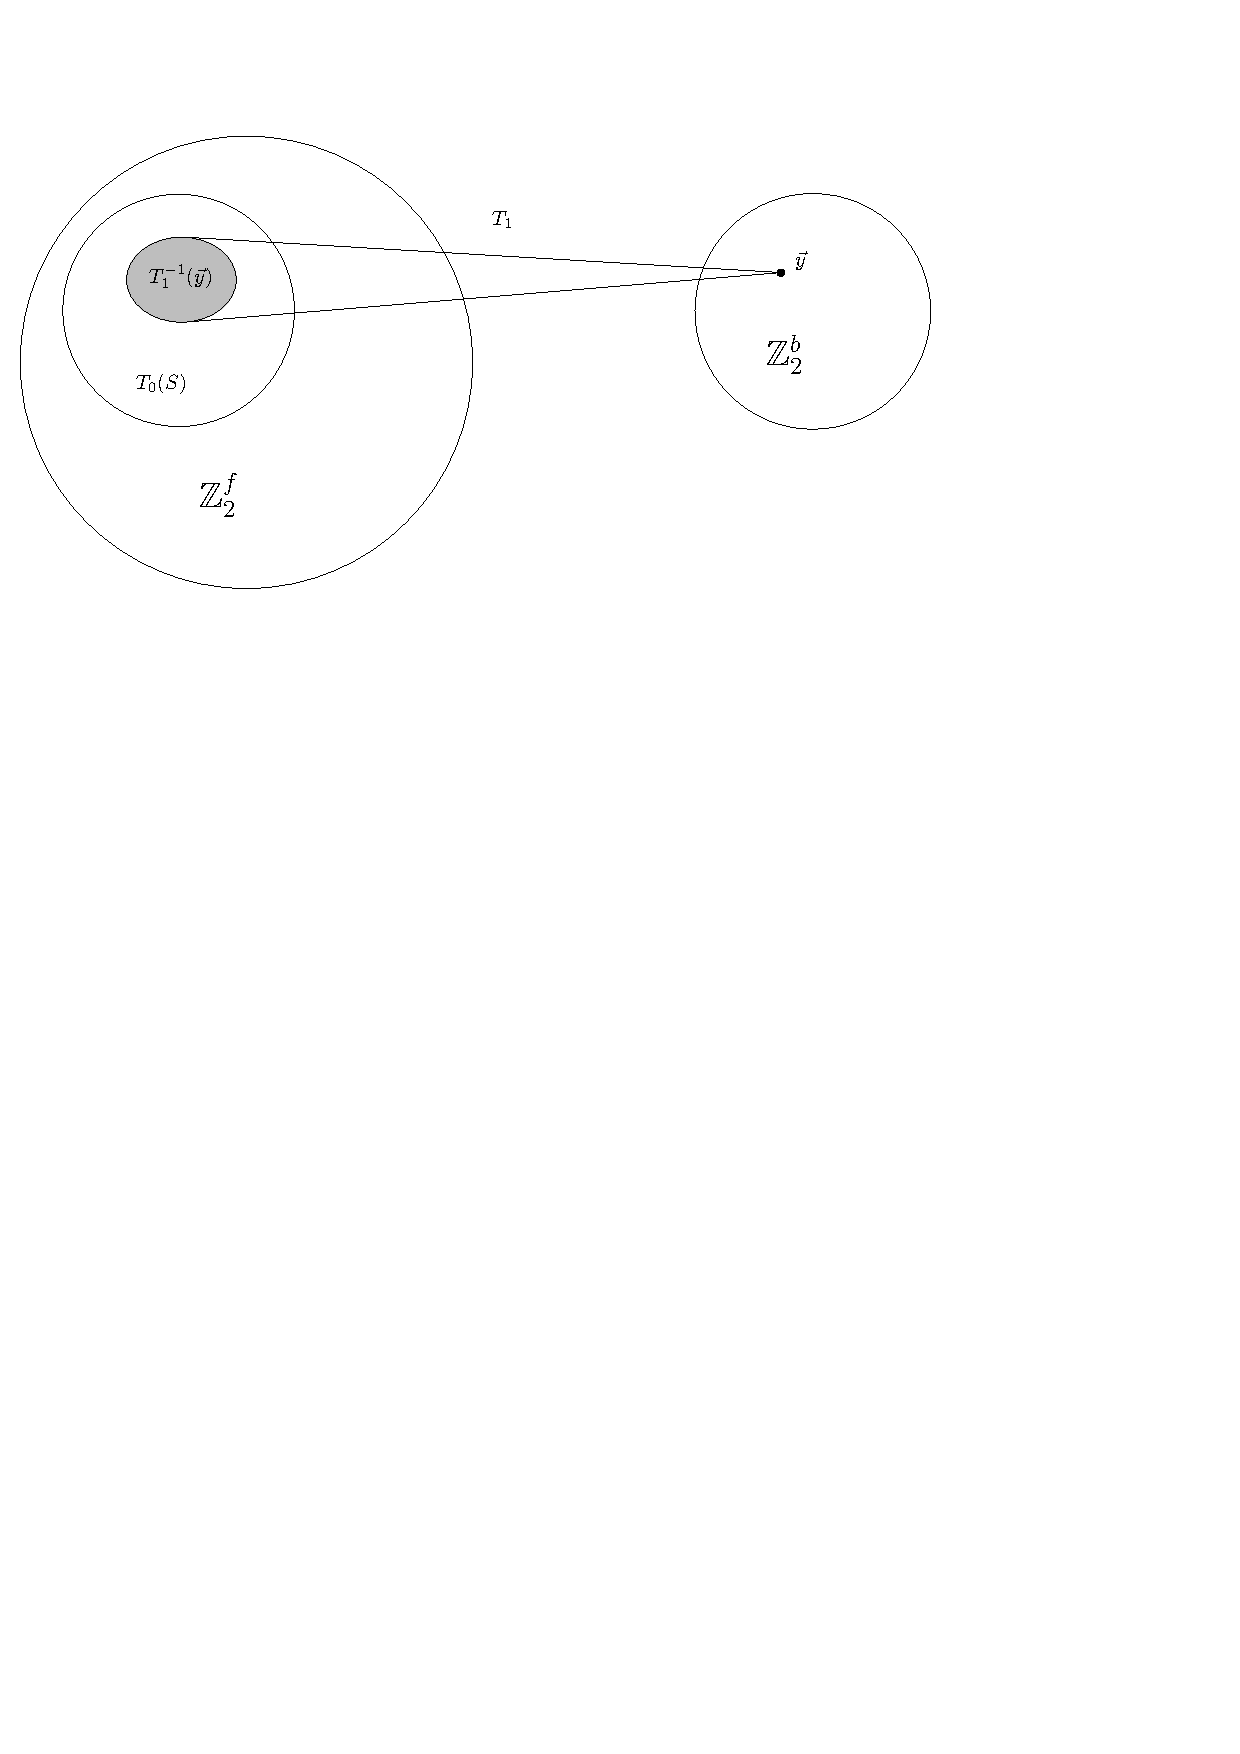
\includegraphics[width=0.7\textwidth]{images/e2}

  \caption{Occurrence of the event $E_2$.}
\end{figure}

\end{proof}

Now we use the previous equivalency to estimate the probability of the event $E_2$ as stated in the following remark. 
\begin{remark}
\label{remark-e2-probability}
Let $T_0: \vecspace{u} \rightarrow \vecspace{f}$, $T_1: \vecspace{f} \rightarrow \vecspace{b}$ be linear transformations with $T_1$ being surjective and $S \subset U$. Set $d = \frac{|\vecspace{f}|}{|S|}$. If $|S| \leq b2 ^ b$ and $d > 1$, then 
\[
	\Prob{E_2(S, T_0, T_1))} \leq d^{-\log d - \log \log d} \text{.}
\]
\end{remark}
\begin{proof}
We apply Theorem \ref{theorem-linear-function-set-onto} for the transformation $T_1$, the set $\vecspace{f} - T_0(S)$, the target space $\vecspace{b}$ and the inverse density $\mu = 1 - \frac{|\vecspace{f} - T_0(S)|}{|\vecspace{f}|}$ and obtain
\[
	\Prob{T_1(\vecspace{f} - T_0(S)) \neq \vecspace{b}} \leq \mu ^ {f - b - \log b + \log \log \frac{1}{\mu}} \text{.}
\]

We can estimate $\mu$ using only the value $d$ as
\[
	\mu = 1 - \frac{|\vecspace{f} - T_0(S)|}{|\vecspace{f}|} = 1 - \frac{|\vecspace{f}| - |T_0(S)|}{|\vecspace{f}|} = \frac{|T_0(S)|}{|\vecspace{f}|} \leq \frac{|S|}{|\vecspace{f}|} = \frac{1}{d} < 1 \text{.}
\]
To obtain the bound claimed by the remark rewrite the logarithm of the value $d$,
\[
	\log d = \log \frac{|\vecspace{f}|}{|S|} = \log |\vecspace{f}| - \log |S| \geq \log |\vecspace{f}| - \log (b 2 ^ b) = f - b - \log b \text{.}
\]

In the following computation we use Corollary \ref{corollary-f0} to remove the inverse density $\mu$. Since $E_2 \equiv T_1(\vecspace{f} - T_0(S)) \neq \vecspace{b}$ and $\mu \leq \frac{1}{d}$ we have the needed bound,
\[
\begin{split}
\Prob{E_2}
	& \leq \mu^{f - b - \log b + \log \log \left(\frac{1}{\mu}\right)} \\
	& \leq \mu ^ {\log d + \log \log \left(\frac{1}{\mu}\right)} \\
	& \leq \left(\frac{1}{d}\right) ^ {\log d + \log \log d} \\
	& = d ^ {-\log d - \log \log d} \text{.} \\
\end{split}
\]

To meet the assumptions of Theorem \ref{theorem-linear-function-set-onto}, we must have that $\emptyset \neq \vecspace{f} - T_0(S)$ and $\vecspace{f} - T_0(S) \neq \vecspace{f}$. Since the $S \neq \emptyset$, it certainly holds that $\vecspace{f} - T_0(S) \neq \vecspace{f}$. Because $d = \frac{|\vecspace{f}|}{|S|} > 1$, it follows that $|\vecspace{f}| > |S| \geq |T_0(S)|$ and the set $\vecspace{f} - T_0(S)$ then can not be empty.
\end{proof}

We show similar remarks fitting the situation when the size of the set $S$ is proportional to that of the target space $\vecspace{b}$. This corresponds to the situation when hashing only $\alpha m$ elements.

\begin{statement}
\label{statement-e2-probability-linear-good}
Let $T_0: \vecspace{u} \rightarrow \vecspace{f}$, $T_1: \vecspace{f} \rightarrow \vecspace{b}$ be linear transformations with $T_1$ being surjective and $S \subset U$. Let $\alpha \in \mathbb{R}$, $\alpha > 0$ and assume that $|S| = \alpha 2 ^ b$.
\begin{enumerate}
\item If $d = \frac{2 ^ f}{\alpha b 2 ^ b}$ and $d > 1$, then $\Prob{E_2(S, T_0, T_1))} \leq d ^ {-\log \alpha - \log d - \log \log d}$.
\item If $d = \frac{2 ^ f}{\alpha 2 ^ b}$ and $d > 1$, then $\Prob{E_2(S, T_0, T_1))} \leq d ^ {\log b - \log \alpha - \log d - \log \log d}$.
\end{enumerate}
\end{statement}
\begin{proof}
We slightly changed the choice of the variable $d$ and naturally moved to a different size $|S|$. In original Remark \ref{remark-e2-probability} we have $d = \frac{|A|}{|S|}$. In fact, we needed just three inequalities concerning $d$
\begin{enumerate}
\item [(1)] $d > 1$,
\item [(2)] $\mu = 1 - \frac{|A - T_0(S)|}{|A|} \leq \frac{1}{d} < 1$,
\item [(3)] $\log d \geq f - b - \log b$.
\end{enumerate}

First, we try to verify them. The first is an assumption of the statement. The second one follows from $d > 1$
\[
	\mu = 1 - \frac{|\vecspace{f} - T_0(S)|}{|\vecspace{f}|} = \frac{|T_0(S)|}{|\vecspace{f}|} \leq \frac{|S|}{|\vecspace{f}|} = \frac{\alpha |\vecspace{b}|}{|\vecspace{f}|} \leq 
\begin{cases}
\frac{\alpha b 2 ^ b}{2 ^ f} = \frac{1}{d} < 1 & \text{if } d = \frac{2 ^ f}{\alpha b 2 ^ b} \\
\frac{\alpha 2 ^ b}{2 ^ f} = \frac{1}{d} < 1 & \text{if } d = \frac{2 ^ f}{\alpha 2 ^ b} \text{.}
\end{cases}
\]

If we do not place any additional bound on the value $\alpha$ we can not get the third inequality exactly. In the first case if $d = \frac{2 ^ f}{\alpha b 2 ^ b}$, we have 
\[
	\log d = f - \log \alpha - b - \log b \text{.}
\]
In the second case if $d = \frac{2 ^ f}{\alpha 2 ^ b}$, then
\[
	\log d = f - \log \alpha - b \text{.}
\]

Recall that from the first two inequalities if follows that the assumptions of Theorem \ref{theorem-linear-function-set-onto} are met
\begin{gather*}
\emptyset \neq \vecspace{f} - T_0(S) \neq \vecspace{f} \text{,} \\
\mu < 1 \text{.}
\end{gather*}
Now we use the theorem again for the transformation $T_1$, the set $\vecspace{f} - T_0(S)$ and the inverse density $\mu$ and obtain
\[
	\Prob{E_2} \leq \mu ^ {f - b - \log b - \log \log \left( \frac{1}{\mu} \right)} \text{.}
\]

To prove the statement perform a similar estimation as in the original proof. For the next estimates use Corollary \ref{corollary-f0} and the fact that $\mu \leq \frac{1}{d}$. For the first case it follows that
\[
\begin{split}
\Prob{E_2} 
	& \leq \mu ^ {f - b - \log b + \log \log \left( \frac{1}{\mu} \right)} \\
	& \leq \mu ^ {\log d + \log \alpha + \log \log \left( \frac{1}{\mu} \right)} \\
	& \leq \left(\frac{1}{d}\right) ^ {\log d + \log \alpha + \log \log d} \\
	& = d ^ {-\log \alpha - \log d - \log \log d} \text{.}
\end{split}
\]
In the second case we have that 
\[
\begin{split}
\Prob{E_2} 
	& \leq \mu ^ {f - b - \log b + \log \log \left( \frac{1}{\mu} \right)} \\
	& \leq \mu ^ {\log d + \log \alpha - \log b  + \log \log \left( \frac{1}{\mu} \right)} \\
	& \leq \left(\frac{1}{d}\right) ^ {\log d + \log \alpha - \log b + \log \log d} \\
	& = d ^ {- \log b -\log \alpha - \log d - \log \log d} \text{.}
\end{split}
\]
\end{proof}

A similar remark for an estimate of the conditional probability of the event $E_2 \mid E_1$ now follows.
\begin{remark}
\label{remark-prob-l-length-chain}
Let $T_0: \vecspace{u} \rightarrow \vecspace{f}$ and $T_1: \vecspace{f} \rightarrow \vecspace{b}$ be random uniformly chosen linear transformations with $T_1$ being surjective and $T = T_1 \circ T_0$. Let $S \subset \vecspace{u}$, $\epsilon \in (0, 1)$ and $l \in \mathbb{N}$, $l \geq c_{\epsilon}(f - b)2 ^ {f - b}$ where constant $c_\epsilon$ is from Theorem \ref{theorem-linear-function-set-onto}. Then
\[
	\Prob{E_2(S, T_0, T_1) \mid E_1(S, T, l)} \geq 1 - \epsilon \text{.}
\]
\end{remark}
\begin{proof}
According to Model \ref{remark-model-uniform-linear-map-selection} we have that the linear transformation $T = T_1 \circ T_0$ is chosen uniformly.

Assume that the event $E_1$ occurs. So there is a maximal subset $S_A \subseteq S$, $|S_A| > l$ mapped to a singleton $\vec{y} \in \vecspace{b}$. We fix the vector and define $U_A = T^{-1}(\vec{y})$ and $F_A = T_1^{-1}(\vec{y})$. Notice that $S_A = U_A \cap S$. According to Lemma \ref{lemma-linear-transformation-domain-distribution} the sets $U_A$ and $F_A$ are affine vector subspaces and $|F_A| = 2 ^ {f - b}$.

Since $T_0$ is a random uniformly chosen linear mapping from Model \ref{remark-model-uniform-linear-map-selection-affine} it follows that its restriction $T_0|_{U_A}$ is also a random uniformly chosen affine linear transformation.

Now we use Corollary \ref{corollary-affine-e2} for the source space $U_A$, the set $S_A \subseteq U_A$, the target space $F_A$ and mapping $T_0|_{U_A}$ and obtain that 
\[
	\Prob{T_0|_{U_A}(S_A) = F_A \mid E_1} \geq 1 - \epsilon \text{.}
\]

If $F_A = T_1^{-1}(\vec{y}) \subseteq T_0(S)$, then the event $E_2$ certainly occurs. Stated in the language of probability:
\[
	\Prob{F_A \subseteq T_0(S) \mid E_1} \leq \Prob{E_2 \mid E_1} \text{.}
\]

From $F_A = T_0|_{U_A}(S) \subseteq T_0(S)$ it follows that:
\[
	\Prob{E_2 \mid E_1} \geq \Prob{F_A \subseteq T_0(S) \mid E_1} \geq \Prob{F_A = T_0|_{U_A}(S_A) \mid E_1} \geq 1 - \epsilon \text{.}
\]

Thus the remark's proof is finally finished.

\begin{figure}
  \centering
    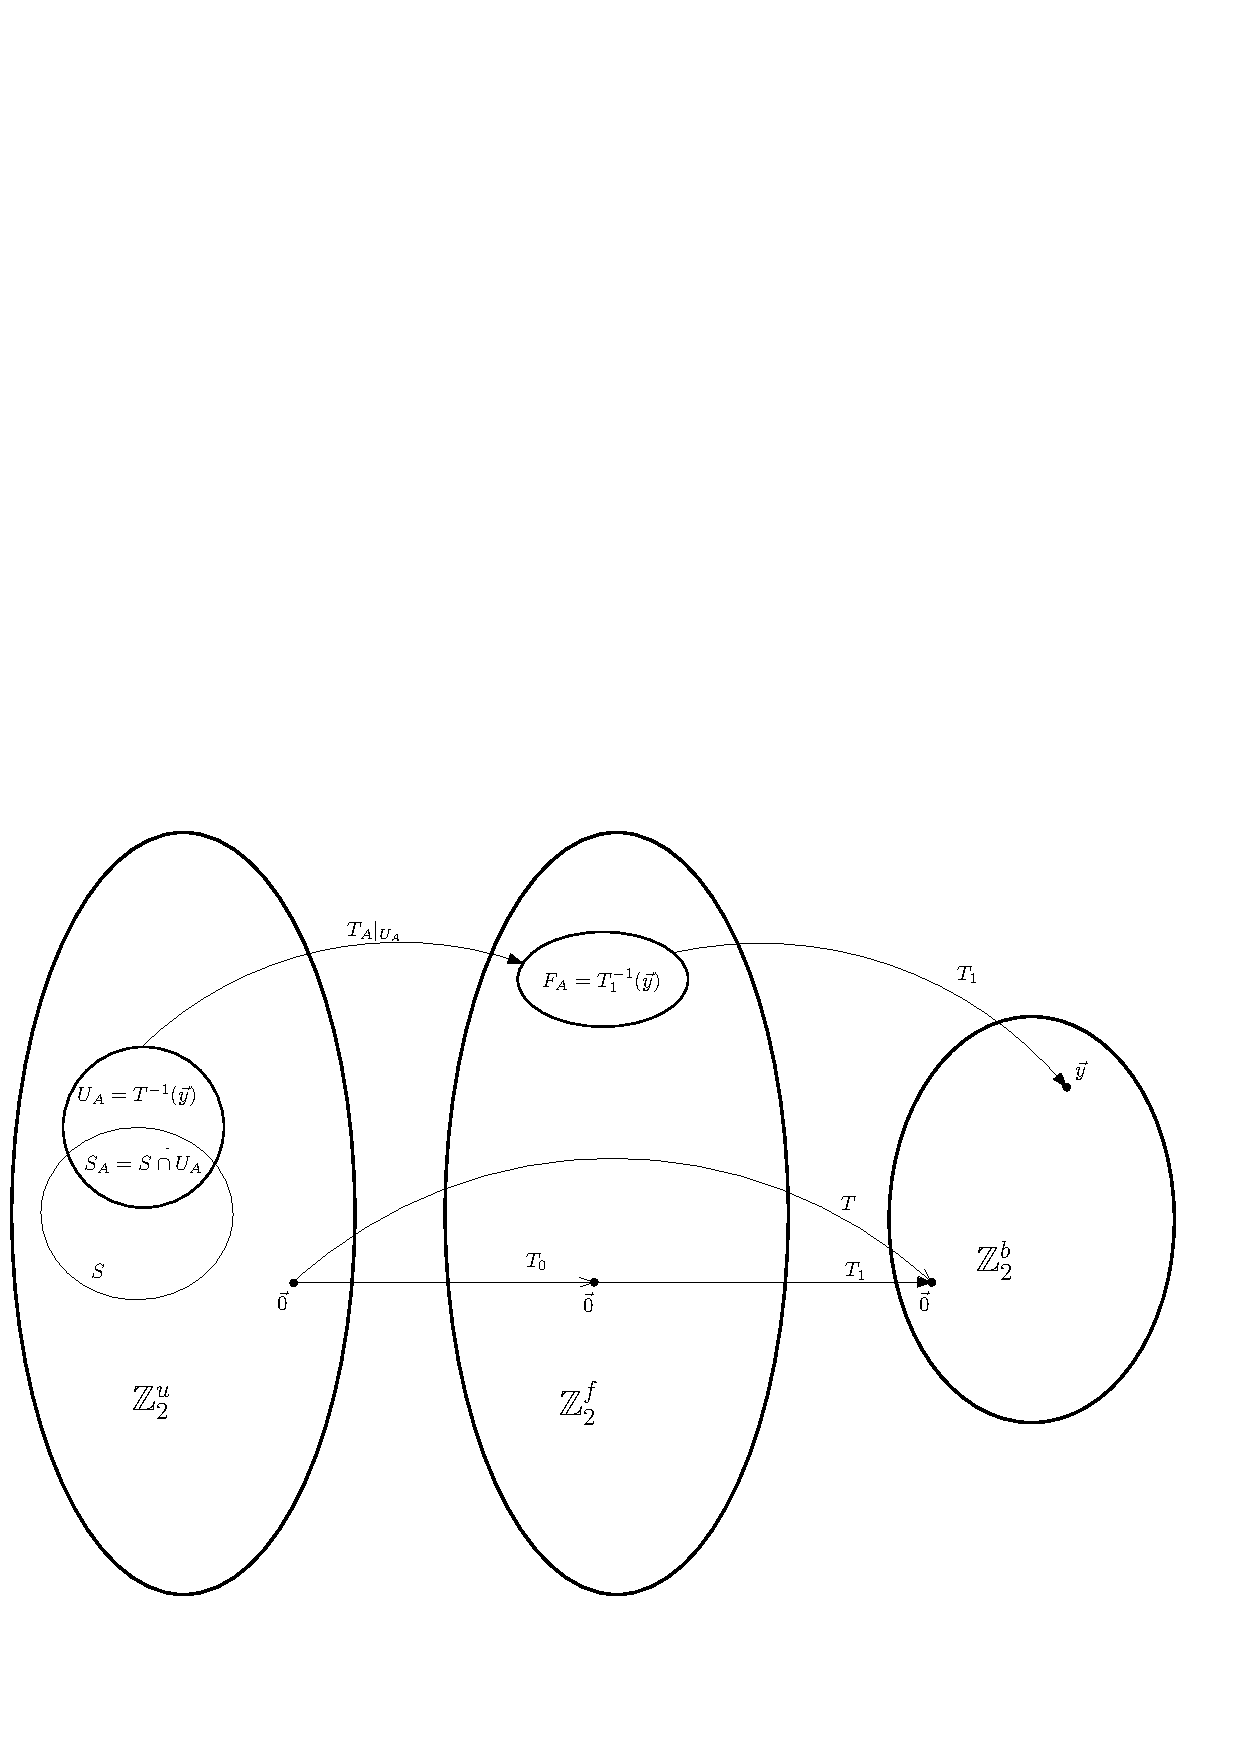
\includegraphics[width=0.9\textwidth]{images/elpsl_proof}
  \caption{Image depicting the situation in the proof.}
\end{figure}

\end{proof}

The next corollary puts the previous claims together.
\begin{corollary}
\label{corollary-prob-e2-e1}
Let $T_0: \vecspace{u} \rightarrow \vecspace{f}$ and $T_1: \vecspace{f} \rightarrow \vecspace{b}$ be a random uniformly chosen linear transformations with $T_1$ being surjective. Let $\epsilon \in (0, 1)$, $S \subset \vecspace{u}$ and $l \in \mathbb{N}$, $l \geq c_{\epsilon}(f - b)2 ^ {f - b}$. Then
\[
	\Prob{E_1(S, T, l)} \leq \frac{1}{1 - \epsilon} \Prob{E_2(S, T_0, T_1)} \text{.}
\]
\end{corollary}
\begin{proof}
The proof is a straightforward use of the previous remark and Lemma \ref{lemma-conditional-probability-event-estimate}. They imply that
\[
	\Prob{E_1} \leq \frac{\Prob{E_2}}{\Prob{E_2 \mid E_1}} \leq \frac{1}{1 - \epsilon}\Prob{E_2} \text{.}
\]
\end{proof}

Definition \ref{definition-lpsl} of the variable $\lpsl$ comes from the area of hashing and uses the notation of chains and their lengths. However we can refer to it now, too. Assume that the universe is equal to the vector space $\vecspace{u}$ and the hash table is represented by the vector space $\vecspace{b}$ and $S \subset U$. The randomness is brought by the uniform choice of linear transformation $T: \vecspace{u} \rightarrow \vecspace{b}$ among $LT(\vecspace{u}, \vecspace{b})$. Realise that the random variable $\psl(\vec{b})~=~|T^{-1}(\vec{b}) \cap S|$ for a vector $\vec{b} \in \vecspace{b}$. By setting $\lpsl = \displaystyle\max_{\vec{b} \in \vecspace{b}} \psl(\vec{b})$ their meanings remain the same. 

\begin{lemma}
\label{lemma-e1-lpsl-equivalence}
If $T: \vecspace{u} \rightarrow \vecspace{b}$ is a random uniformly chosen linear transformation, $S \subset \vecspace{u}$ and $l \in \mathbb{N}$, then $E_1(S, T, l) \Leftrightarrow \lpsl > l$.
\end{lemma}
\begin{proof}
The event $E_1(S, T, l)$ denotes the existence of a vector $\vec{y} \in \vecspace{b}$ such that $|T^{-1}(\vec{y}) \cap S| > l$. Observe that such vector $\vec{y}$ exists if and only if the variable $\lpsl > l$ because
\[
(\exists \vec{y} \in \vecspace{b}: |T^{-1}(\vec{y}) \cap S| > l) \Leftrightarrow (\exists \vec{y} \in \vecspace{b}: \psl(\vec{y}) > l) \Leftrightarrow (\lpsl > l) \text{.}
\] 
\end{proof}

We are able to bound the probability density function of the random variable $\lpsl$ when referring to its above definition.
\begin{remark}
\label{remark-probability-long-chain}
Let $T: \vecspace{u} \rightarrow \vecspace{b}$ be a random uniformly chosen linear map, $\epsilon \in (0, 1)$ and $S \subset \vecspace{u}$, $|S| \leq b 2 ^ b$. Then for every $r \geq 4$
\[
	\Prob{\lpsl > 4 c_\epsilon r b \log b} \leq \frac{1}{1 - \epsilon} \left(\frac{r}{\log r}\right)^{-\log \left(\frac{r}{\log r}\right) - \log \log \left(\frac{r}{\log r}\right)} \text{.}
\]
\end{remark}
\begin{proof}
In the proof we just conveniently use the previous remarks. We only have to choose their parameters. First we create a factor space $\vecspace{f}$, its dimension is specified later. From Model \ref{remark-model-uniform-linear-map-selection-affine} and the random uniform and independent selection of two linear transformations $T_0: \vecspace{u} \rightarrow \vecspace{f}$ and surjective $T_1: \vecspace{f} \rightarrow \vecspace{b}$ it follows that the linear mapping $T: \vecspace{u} \rightarrow \vecspace{b}$ such that $T = T_1 \circ T_0$ is chosen uniformly as well. Fix the mappings $T_0$, $T_1$ and $T$.

Now set 
\[
\begin{split}
	f & = \left\lfloor b + \log b + \log r - \log \log r + 1 \right\rfloor \text{,} \\
	l & = 4c_{\epsilon}r b \log b \text{,} \\
	d & = \frac{2 ^ f}{|S|} \geq \frac{2 ^ f}{b 2 ^ b} \geq \frac{b 2 ^ b}{b 2 ^ b} \cdot \frac{r}{\log r} = \frac{r}{\log r} \geq 2 \text{.}
\end{split}
\]
The choice of $f$ implies that $|\vecspace{f}| \geq \vecspace{b}|$ because 
\[ 
f \geq b + \log b + \log r - \log \log r \geq b \text{.}
\]
Hence a surjective function $T_1$ exists and may be fixed. Notice that the choices meet all the assumptions, $d > 1$, of Remark \ref{remark-e2-probability}. To verify the condition $l \geq c_\epsilon (f - b) 2 ^ {f - b}$ of Remark \ref{remark-probability-long-chain} we first show that
\[
	2 ^ {f - b} \leq 2 ^ {b + \log b + \log r - \log \log r + 1 - b} = \frac{2 r b}{\log r} \text{.}
\]
From the fact, $f - b \leq \log \left(\frac{2 r b}{\log r}\right) \leq 2 \log b \log r$, we have that the assumption holds since
\[
\begin{split}
c_{\epsilon}(f - b) 2 ^ {f - b}
	& \leq c_{\epsilon} \frac{2 r b}{\log r} \log \left(\frac{2 r b}{\log r}\right) \\
	& \leq 4 c_{\epsilon} b \frac{r}{\log r} \log b \log r \\
	& = 4 c_{\epsilon} r b \log b \\
	& = l \text{.}
\end{split}
\]

From Corollary \ref{corollary-prob-e2-e1}, Remark \ref{remark-e2-probability} and Corollary \ref{corollary-f1} it follows that
\[
\begin{split}
\Prob{E_1}
	& \leq \frac{1}{1 - \epsilon} \Prob{E_2} \\
	& \leq \frac{1}{1 - \epsilon} d ^ {-\log d - \log \log d} \\ 
	& \leq \frac{1}{1 - \epsilon} \left(\frac{r}{\log r}\right)^{-\log \left(\frac{r}{\log r}\right) - \log \log \left(\frac{r}{\log r}\right)} \text{.}
\end{split}
\]

According to Lemma \ref{lemma-e1-lpsl-equivalence} the event $E_1$ occurs if and only if $\lpsl > l$. The proof is completed by writing down the facts obtained so far
\[
\begin{split}
\Prob{\lpsl > l} 
	& = \Prob{\lpsl > 4c_{\epsilon} r b \log b} \\
	& = \Prob{E_1(S, T, 4c_{\epsilon} r b \log b)} \\
	& \leq \frac{1}{1 - \epsilon} \left(\frac{r}{\log r}\right)^{-\log \left(\frac{r}{\log r}\right) - \log \log \left(\frac{r}{\log r}\right)} \text{.}
\end{split}
\]
\end{proof}

We modify the previous remark for the set $S$ having $|S| = \alpha 2 ^ b$.
\begin{remark}
\label{remark-lpsl-pdf-linear-amount}
Let $T: \vecspace{u} \rightarrow \vecspace{b}$ be a random uniformly chosen linear mapping, $\epsilon \in (0, 1)$, $r \geq 4$ and $\alpha \in (0.5, \frac{\log r}{2})$. If $S$ is a subset of $\vecspace{u}$ such that $|S| = \alpha 2 ^ b$, then
\[
\begin{split}
& \Prob{\lpsl > 4 c_\epsilon \alpha r b \log b} \leq \frac{1}{1 - \epsilon} \left(\frac{r}{\log r}\right)^{-\log \alpha - \log \left(\frac{r}{\log r}\right) - \log \log \left(\frac{r}{\log r}\right)} \text{and} \\
& \Prob{\lpsl > 2 \alpha c_\epsilon r} \leq \frac{1}{1 - \epsilon}\left(\frac{r}{\log r}\right)^{\log \log m - \log \alpha - \log \left(\frac{r}{\log r}\right) - \log \log \left(\frac{r}{\log r}\right)} \text{.}
\end{split}
\]
\end{remark}
\begin{proof}
We do not repeat the whole proof of Remark \ref{remark-probability-long-chain} since the approach remains the same. Like in the previous proof, fix the linear mappings $T_0$, surjective $T_1$ with $T = T_1 \circ T_0$ and let $\vecspace{f}$ be the factor space. We just show the choices that prove the remark. The choices for the first claim are indexed with $1$ and in the second case we use the index $2$. When we refer to a chosen variable without an index, then the statement, in which it appears, must be valid for either choice.
Now perform the choices by setting
\[
\begin{split}
	f_1 & = \left\lfloor b + \log b + \log r - \log \log r + \log \alpha + 1 \right\rfloor \text{,} \\
	f_2 & = \left\lfloor b + \log r - \log \log r + \log \alpha + 1 \right\rfloor \text{,} \\
	d_1 & = \frac{2 ^ {f_1}}{\alpha b 2 ^ b} \text{,} \\
	d_2 & = \frac{2 ^ {f_2}}{\alpha 2 ^ b} \text{,} \\
	l_1 & = 4 c_\epsilon \alpha r b \log b \text{,} \\
	l_2 & = 2 \alpha c_\epsilon r \text{.}
\end{split}
\]

So that $T_1$ exists, we have to verify that $|\vecspace{f}| \geq |\vecspace{b}|$. It is enough to have $f \geq b$. The inequality $f \geq b$ follows from the fact $\log r - \log \log r + \log \alpha \geq 0$ and from our choice of $f$ since
\[
\begin{split}
	f_1 & \geq b + \log b + \log r - \log \log r + \log \alpha \geq b \text{,} \\
	f_2 & \geq b + \log r - \log \log r + \log \alpha \geq b \text{.}
\end{split}
\]

Secondly, we show that the assumptions of Statement \ref{statement-e2-probability-linear-good} are met for both choices of $d$. Precisely we need $d > 1$ and this is satisfied because
\[
\begin{split}
& d_1 = \frac{2 ^ {f_1}}{\alpha b 2 ^ b} \geq \frac{r}{\log r} \geq 2 \text{,} \\
& d_2 = \frac{2 ^ {f_2}}{\alpha 2 ^ b} \geq \frac{r}{\log r} \geq 2 \text{.}
\end{split}
\]

Naturally, we want to meet the condition placed on the variable $l$ of Corollary \ref{corollary-prob-e2-e1}. Recall the assumption $\alpha < \frac{\log r}{2}$ that is used in either case. Let us discuss the first case
\[ 
	f_1 - b \leq \log b + \log r - \log \log r + \log \alpha + 1 \leq \log b + \log r \leq 2 \log b \log r \text{.} 
\] Thus for the value of the variable $l_1$ we have that 
\[
\begin{split}
c_{\epsilon} (f_1 - b) 2 ^ {f_1 - b}
	& < c_{\epsilon} \left(\frac{2 \alpha b r}{\log r} \right) \left(2 \log b \log r \right) \\
	& \leq 4 c_{\epsilon} \alpha r b \log b \\
	& = l_1 \text{.}
\end{split}
\]
The validity in the second case follows from
\[
\begin{split}
c_\epsilon (f_2 - b) 2 ^ {f_2 - b}
	& \leq c_\epsilon \left(\frac{2 \alpha r}{\log r}\right) \log \left( \frac{2 \alpha r}{\log r} \right) \\
	& \leq 2 c_\epsilon \alpha \frac{r}{\log r} \log r \\
	& = 2 c_\epsilon \alpha r = l_2 \text{.}
\end{split}
\]


Thus we are able to refer to Corollary \ref{corollary-prob-e2-e1}. Now use Lemma \ref{lemma-e1-lpsl-equivalence}, Corollary \ref{corollary-prob-e2-e1}, Remark \ref{remark-e2-probability} and Corollary \ref{corollary-f1} in either case. In the first one we have
\[
\begin{split}
\Prob{\lpsl > 4 c_{\epsilon} \alpha r b \log b} 
	& = \Prob{\lpsl > l_1} \\
	& = \Prob{E_1(S, T, l_1)} \\
	& \leq \frac{1}{1 - \epsilon}{\Prob{E_2}} \\
	& \leq \frac{1}{1 - \epsilon} d ^ {-\log \alpha - \log d - \log \log d} \\
	& = \frac{1}{1 - \epsilon} \left(\frac{r}{\log r}\right)^{-\log \alpha - \log \left(\frac{r}{\log r}\right) - \log \log \left(\frac{r}{\log r}\right)} \text{.}
\end{split}
\]
And in the second case we have
\[ 
\begin{split}
\Prob{\lpsl > 2 \alpha c_\epsilon r} 
	& = \Prob{\lpsl > l_2} \\
	& = \Prob{E_1(S, T, l_2)} \\
	& \leq \frac{1}{1 - \epsilon}{\Prob{E_2}} \\
	& \leq \frac{1}{1 - \epsilon} d ^ {\log b - \log \alpha - \log d - \log \log d} \\
	& \leq \frac{1}{1 - \epsilon} \left(\frac{r}{\log r}\right)^{\log b - \log \alpha - \log \left(\frac{r}{\log r}\right) - \log \log \left(\frac{r}{\log r}\right)} \text{.}
\end{split}
\]
\end{proof}

\begin{section}{The original result}
The last two theorems of the previous chapter give us enough power to achieve our goal - asymptotic restriction of the worst case chain length. Once again we achieve this limit when hashing even super-linear amount of $n \log n$ elements into $n$ slots. By hashing a linear amounts this expected length can not grow. Every hashed set can be extended into $n \log n$ elements and the estimate must still remain valid. 

The most common models use load factors lower than one. Because of these models we generalise theorem so that it is parametrised by the table's load factor. Important relation of the expected length of the longest chain on the table's load factor is found. The result is that the multiplicative constant of the asymptotic growth is relative to the load factor of a hash table. New results are achieved by modifications of the given proofs with some new ideas.

\begin{theorem}
\label{theorem-n-logn-to-n}
Let $U = \vecspace{w}$ be the hashed universe, $B = \vecspace{t}$ be the hash table and $S \subset U$ be the hashed set such that $|S| = m \log m$ where $t \in \mathbb{N}, m = 2 ^ t$. Let $H = LT(\vecspace{w}, \vecspace{t})$ be the universal system used. Then 
\[
	\Expect{\lpsl} \in O(\log m \log \log m) \text{.}
\]
\end{theorem}
The original proof is showed in the following few pages. It contains some remarks and definitions that are pointed out on their own and later refined. It uses two basic ideas; factorisation and probability estimates of two correlated events.

Let the target space, representation of the hash table, be denoted by $B = \vecspace{t}$. As in the previous proof we will factor a linear transformation $T \in H$, $T: \vecspace{w} \rightarrow \vecspace{t}$. We define factor vector space $A = \vecspace{u}$ for $u \geq \log n$ and two functions $T_0: \vecspace{w} \rightarrow \vecspace{u}$ and $T_1: \vecspace{u} \rightarrow \vecspace{t}$ which is surjective. Both linear functions $T_0$ and $T_1$ are selected uniformly among $LT(U, A)$ and $LTS(A, B)$ respectively. By direct use of model \ref{remark-model-uniform-linear-map-selection} we obtain uniform choice of the transformation $T = T_1 \circ T_0$ .

The second idea of the proof is to estimate the probability of event called $E1$, $\lpsl > l$, for any natural number $l$. The probability bound on $E_1$ is found by inspecting another quite unnatural event $E_2$. Probability of event $E_1$ is then simply determined by discovering the probabilities $\Prob{E_2 | E_1}$ and $\Prob{E_2}$.

\begin{definition}
Let $l$ be a natural number, $T: U \rightarrow B$ be a linear transformation and $S \subset U$ be the hashed set. Event $E_1(S, T, l)$ denotes existence of a chain of length at least $l$ elements when using function $T$. 
\[ 
	E_1(S, T, l) \equiv \exists \vec{y} \in B: | T^{-1}(\vec{y}) \cap S | > l
\]
\end{definition}

\begin{definition}
Let $T_0: U \rightarrow A, T_1: A \rightarrow B$ be linear transformations where $T_2$ is surjective and $S \subset U$ be the hashed set. Event $E_2(S, T_0, T_1)$ is then defined as:
\[
	E_2(S, T_0, T_1) \equiv \exists \vec{y} \in B: T_1^{-1}(\vec{y}) \subseteq T_0(S) \text{.}
\]
\end{definition}

When it is clear what we mean by $S, T_0, T_1$ and $t$ we omit the parametrisation of the events and just use $E_1$ or $E_2$.

Now we will point out another definition of the event $E_2$ that fits better to the scheme of remark $\ref{theorem-linear-function-set-onto}$.
\begin{remark}
\label{remark-e2-equivalency}
Let $T_0: U \rightarrow A$ and $T_1: A \rightarrow B$ be linear transformations and moreover $T_2$ be surjective. Let $S \subset U$ be the hashed set. Appearance of event $E_2(S, T_0, T_1)$ is then equivalent to
\[
	E_2(S, T_0, T_1) \equiv \exists \vec{y}: T_1^{-1}(\vec{y}) \subseteq T_0(S) \Leftrightarrow T_1(A - T_0(S)) \neq B \text{.}
\]
\end{remark}
\begin{proof}
To proof direction from the left to the right assume that event $E_2$ is present. Event $E_2$ occurs if and only if there is a vector $\vec{y} \in B$ such that $T_1^{-1}(\vec{y}) \subseteq T_1(S)$. Under these conditions transformation $T_1$ may not display set $A - T_0(S)$ onto $B$ since $\vec{y} \notin T_1(A - T^{-1}(y)) \supseteq T_1(A - T_0(S))$ or equivalently $B \neq T_1(A - T_0(S))$.

If $B \neq T_1(A - T_0(S))$ then there exists a vector $\vec{y} \in B$ such that $\vec{y} \notin T_1(A - T_0(S))$. Since $T_1$ is surjective we have $T_1(A) = B$. Because no point from $A - T_0(S)$ is displayed on $\vec{y}$ the whole preimage of $\vec{y}$ must be contained in $T_0(S)$, $T_1^{-1}(\vec{y}) \subseteq T_0(S)$.
\end{proof}

As mentioned before we can use the previous equivalency to estimate probability of event $E_2$ as stated in the following remark. 
\begin{remark}
\label{remark-e2-probability}
Let $U = \vecspace{w}$, $A = \vecspace{u}$ and $B = \vecspace{t}$. Let $T_0: U \rightarrow A$ and $T_1: A \rightarrow B$ be linear transformations where $T_1$ is surjective and $S \subset U$ denote the hashed set such that $|S| \leq |B| \log |B|$. Define $d = \frac{|A|}{|S|}$. If $d > 1$ then 
\[
	\Prob{E_2(S, T_0, T_1))} \leq d^{-\log d - \log \log d} \text{.}
\]
\end{remark}
\begin{proof}
Theorem \ref{theorem-linear-function-set-onto} for surjective transformation $T_1$, set $A - T_0(S) \subset A$, target space $B = \vecspace{t}$ and $\mu = \frac{|T_0(S)|}{|A|}$ states that
\[
	\Prob{T_1(A - T_0(S)) \neq B} \leq \mu ^ {u - t - \log t + \log \log \frac{1}{\mu}} \text{.}
\]

Corresponding inverse density $\mu$ can be computed as 
\[
	\mu = 1 - \frac{|A - T_0(S)|}{|A|} = 1 - \frac{|A| - |T_0(S)|}{|A|} = \frac{|T_0(S)|}{|A|} \leq \frac{|S|}{|A|} = \frac{1}{d} < 1 \text{.}
\] 

Now we can rewrite logarithm of variable $d$ as 
\[
	\log d = \log \frac{|A|}{|S|} = \log |A| - \log |S| \geq \log |A| - \log (|B| \log |B|) = u - t - \log t \text{.}
\]

Since $E_2 \equiv T_1(A - T_0(S)) \neq B$ we can conclude
\[
\begin{split}
\Prob{E_2}
	& \leq \mu^{u - t - \log t + \log \log \left(\frac{1}{\mu}\right)} \\
	& \leq \mu ^ {\log d + \log \log \left(\frac{1}{\mu}\right)} \\
	& \leq \left(\frac{1}{d}\right) ^ {\log d + \log \log d} \\
	& = d ^ {-\log d - \log \log d} \text{.} \\
\end{split}
\]

Because of the assumptions of theorem \ref{theorem-linear-function-set-onto} the proof of this remark holds only when $\emptyset \neq A - T_0(S) \neq A$. Since $S$ is non-empty set we can see that $A - T_0(S) \neq A$. Because $d = \frac{|A|}{|S|} > 1$ it must be true that $|A| > |S| \geq |T_0(S)|$ and set $A - T_0(S)$ can not be empty.
\end{proof}

A similar lemma for estimating the conditional probability of event $E_2 | E_1$ follows.
\begin{remark}
\label{remark-prob-l-length-chain}
Let $U = \vecspace{w}$, $A = \vecspace{u}$ and $B = \vecspace{t}$. Let $T_0: U \rightarrow A$ and $T_1: A \rightarrow B$ be random uniformly chosen linear transformations where $T_1$ is surjective. Then for every $0 < \epsilon < 1$ there is a constant $c_{\epsilon} > 0$ such that for every $S \subset U$ denoting the hashed  elements and for every $l \in \mathbb{N}$, $l \geq c_{\epsilon}{\frac{|A|}{|B|}}\log\frac{|A|}{|B|}$ the upper bound for the probability of event $E_2 | E_1$ is
\[
	\Prob{E_2(S, T_0, T_1) | E_1(S, T, l)} \geq 1 - \epsilon \text{.}
\]
\end{remark}
\begin{proof}
Suppose that we are given a mapping $T$ and the event $E_1$ appears. There must be a subset $S' \subseteq S$ consisting of at least $l$ elements mapped by $T$ to a single element $\vec{y} \in B$. We fix this element and define $U' = T^{-1}(\vec{y})$ and $A' = T_1^{-1}(\vec{y})$. Notice that $S' = U' \cap S$.

From lemma \ref{lemma-linear-transformation-domain-distribution} it follows that size of the set $A'$ is exactly $\frac{|A|}{|B|}$. And from lemma \ref{lemma-linear-transformation-domain-distribution} we have that sets $A'$ and $U'$ are affine subspaces. Since $T_0$ is random uniformly chosen linear mapping its restriction $T_0|_{U'}$ is also a random and uniformly chosen linear transformation as stated in model \ref{remark-model-uniform-linear-map-selection-affine}.

Since we assumed presence of $E_1$ cardinality of $S' = U' \cap S$ must be at least $l \geq c_{\epsilon}\frac{|A|}{|B|} \log\frac{|A|}{|B|} = c_{\epsilon}{A'}\log{A'}$. Now we can use theorem \ref{theorem-set-onto-by-linear-transform} for the source space $U'$, set $S' \subseteq U'$, target space $A'$ and mapping $T_0|_{U'}$ and we obtain that 
\[
	\Prob{T_0|_{U'}(S') = A' | E_1} \geq 1 - \epsilon \text{.}
\]

Remark that we used theorem \ref{theorem-set-onto-by-linear-transform} for affine mapping $T_0|_{U'}$. However, we can use the generating mapping of $T_0|_{U'}$, corresponding non-affine subspaces and transform $S'$ to the original non-affine subspace instead.

Event $E_2$ is certainly present whenever $A' \subseteq T_0(S)$. In the language of probability:
\[
	\Prob{A' \subseteq T_0(S) | E_1} \leq \Prob{E_2 | E_1} \text{.}
\]

Finally we can finish the remark's proof
\[
	\Prob{E_2 | E_1} \geq \Prob{A' \subseteq T_0(S) | E_1} \geq \Prob{A' = T_0|_{U'}(S') | E_1} \geq 1 - \epsilon \text{.}
\]
\end{proof}

\begin{corollary}
\label{corollary-prob-e2-e1}
Let $U = \vecspace{w}$, $A = \vecspace{u}$ and $B = \vecspace{t}$. Let $T_0: U \rightarrow A$ and $T_1: A \rightarrow B$ be random uniformly chosen linear transformations where $T_1$ is surjective. Then for every $0 < \epsilon < 1$ there is a constant $c_{\epsilon} > 0$ such that for every $S \subset U$ denoting the hashed  elements and for every $l \in \mathbb{N}$, $l \geq c_{\epsilon}{\frac{|A|}{|B|}}\log\frac{|A|}{|B|}$ for the probability of event $E_1$ we have
\[
	\Prob{E_1(S, T, l)} \leq \frac{1}{1 - \epsilon} \Prob{E_2(S, T_0, T_1)} \text{.}
\]
\end{corollary}
\begin{proof}
The proof is a straightforward use of the previous remark and definition of conditional probability.
\[
	\frac{\Prob{E_2, E_1}}{\Prob{E_1}} = \Prob{E_2 | E_1} \geq 1 - \epsilon
\]

Using the fact $\Prob{E_2} \geq \Prob{E_2, E_1}$ we conclude:
\[
	\Prob{E_1} \leq \frac{1}{1 - \epsilon}\Prob{E_2, E_1} \leq \frac{1}{1 - \epsilon}\Prob{E_2} \text{.}
\]
\end{proof}

The probability bound of existence of a long chain is estimated by the following theorem.
\begin{remark}
\label{remark-probability-long-chain}
Let $U = \vecspace{w}$, $B = \vecspace{t}$ be vector spaces representing the domain ($U$) and the hash table ($B$). Let $T: U \rightarrow B$ be random uniformly chosen linear map and $m = 2 ^ t = |B|$. For every $0 < \epsilon < 1$ and for every $r > 4$ when hashing $S \subset U$, $|S| \leq t 2 ^ t$ following estimate on the length of the longest chain holds.
\[
	\Prob{\lpsl > 4 c_\epsilon r \log m \log \log m} \leq \frac{1}{1 - \epsilon} \left(\frac{r}{\log r}\right)^{-\log \left(\frac{r}{\log r}\right) - \log \log \left(\frac{r}{\log r}\right)} \text{.}
\]
\end{remark}
\begin{proof}
Proof of this remark is a straightforward use of previous remarks, we only have to choose the values of their parameters. As mentioned before we create the factorisation space $A = \vecspace{u}$. By validity of model \ref{remark-model-uniform-linear-map-selection-affine} uniform and independent choice of two random linear transformations $T_0: U \rightarrow A$ and surjective $T_1: A \rightarrow B$ corresponds to the uniform choice $T: U \rightarrow B$ such that $T = T_1 \circ T_0$.

Since $|S| \leq t 2 ^ t$ we have also that $|S| \leq n \log n$. Our choice of $u$ must confirm to $|A| \geq |B|$ since we need a surjective function $T_1$. The choices also satisfy assumptions of the remark \ref{remark-e2-probability} and corollary \ref{corollary-prob-e2-e1}.
\[
\begin{split}
	u & = \left\lfloor \log m + \log \log m + \log r - \log \log r + 1 \right\rfloor \\
	l & = 4c_{\epsilon}r\log m \log \log m \\
\end{split}
\]

Since $r > 4$ we have that $\frac{r}{\log r} > 1$:
\[
	2 ^ u \geq \frac{rm \log m}{\log r} > m \log m \geq 2 ^ t = |B| \text{.}
\]

Hence the condition $d = \frac{|A|}{|S|} > 1$ of remark \ref{remark-e2-probability} is satisfied because
\[
	d = \frac{|A|}{|S|} = \frac{2^u}{m \log m} \geq \frac{m \log m}{m \log m}\frac{r}{\log r} = \frac{r}{\log r} > 1 \text{.}
\]

Following inequality helps us to prove the assumption $l \geq c_\epsilon \frac{|A|}{|B|} \log \frac{|A|}{|B|}$ of the corollary \ref{corollary-prob-e2-e1}.
\[
	\frac{2^u}{m} \leq \frac{2 ^{\log m + \log \log m + \log r - \log \log r + 1}}{m} = \frac{2 r\log m}{\log r}
\]

Because $\log \left(\frac{2 r\log m}{\log r}\right) \leq 2 \log \log m \log r$ the assumption holds:
\[
\begin{split}
c_{\epsilon}\frac{2^u}{m}\log\left(\frac{2^u}{m}\right)
	& \leq 2 c_{\epsilon} \log m \frac{r}{\log r} \log \left(\frac{2 r\log m}{\log r}\right) \\
	& \leq 4 c_{\epsilon} \log m \frac{r}{\log r} \log \log m \log r \\
	& = 4 c_{\epsilon} r \log m \log \log m \\
	& = l \text{.}
\end{split}
\]

Now using remark \ref{remark-e2-probability} and corollary \ref{corollary-prob-e2-e1} we obtain:
\[
\begin{split}
\Prob{E_1}
	& \leq \frac{1}{1 - \epsilon} \Prob{E_2} \\
	& \leq \frac{1}{1 - \epsilon} d ^ {-\log d - \log \log d} \\ 
	& \leq \frac{1}{1 - \epsilon} \left(\frac{r}{\log r}\right)^{-\log \left(\frac{r}{\log r}\right) - \log \log \left(\frac{r}{\log r}\right)} \text{.}
\end{split}
\]

The event $E_1$ denotes the existence of a chain of size at least $l$ elements. A chain longer than $l$ in a hash table exists if and only if the longest chain is longer than $l$, $\lpsl > l \Leftrightarrow E_1(S, T, l)$. This proof completed by writing down the facts observed so far.

\[
\begin{split}
\Prob{\lpsl > l} 
	& = \Prob{\lpsl > 4c_{\epsilon} r \log m \log \log m} \\
	& = \Prob{E_1(S, T, 4c_{\epsilon} r \log m \log \log m)} \\
	& \leq \frac{1}{1 - \epsilon} \left(\frac{r}{\log r}\right)^{-\log \left(\frac{r}{\log r}\right) - \log \log \left(\frac{r}{\log r}\right)} \\
\end{split}
\]
\end{proof}

Previous claim is very convenient in order to successfully prove theorem \ref{theorem-n-logn-to-n}. For every fixed $0 < \epsilon < 1$ set $K_\epsilon = 4 c_\epsilon \log m \log \log m$.
\[
\begin{split}
\Expect{\lpsl}
	& = \int\limits_0^{\infty} \Prob{\lpsl > r} dr \\
	& \leq 4K_\epsilon + \int\limits_{4K_\epsilon}^\infty \Prob{\lpsl > r} dr \\
	& = 4K_\epsilon + K_\epsilon \int\limits_4^\infty \Prob{\lpsl > rK_\epsilon} dr \\
	& \leq 4K_\epsilon + K_\epsilon \int\limits_4^\infty \frac{1}{1 - \epsilon} \left(\frac{r}{\log r}\right)^{-\log \left(\frac{r}{\log r}\right) - \log \log \left(\frac{r}{\log r}\right)} dr \\
	& = K_\epsilon(4 + I_\epsilon) = O(K_\epsilon) = O(\log m \log \log m)
\end{split}
\]

We substituted $I_\epsilon$ for
\[
I_\epsilon = \int\limits_4^\infty \frac{1}{1 - \epsilon} \left(\frac{r}{\log r}\right)^{-\log \left(\frac{r}{\log r}\right) - \log \log \left(\frac{r}{\log r}\right)} dr \text{.}
\]
The fact that this integral is convergent for every $0 < \epsilon < 1$ is shown later.

The proof of the theorem \ref{theorem-n-logn-to-n} is completed even in more general form. We made no special assumptions on the size of the hashed set $S$ except $|S| \leq |B| \log |B|$. \qed

\mbox{\qedhere}

Multiplicative constant $4 c_\epsilon(4 + I_\epsilon)$ plays an important role for a practical use of this result. In our proofs performed so far we neglected its estimation. We only obtained a good asymptotic result that is negated by the constant's great value. For example when choosing $\epsilon$ equal to $\frac{1}{2}$ only constant $c_\epsilon$ equals $4 ^ {17}$ by usage of the original estimate. Our next goal is to show a better constant's estimate, explore the dependency of the longest chain on load factor of the hash table and find an even better constant when using load factors lower than one.
\end{section}

\begin{section}{Hashing a linear amount of elements with respect to the table's size}
Usage of the hash table with load factors lower than one brings us even lower expected lengths of the longest chains. This situation lowers the multiplicative constant and this is the reason why we examine this case. We already showed if a super-linear amount of elements is hashed then we can expect reasonable worst case behaviour. However the most important is the real expected size of a bucket. Upper bound on the expected operation's running time is equal to $1 + c \alpha$ in every model of universal hashing. So using load factors lower than one has significant impact on the expected case. We must examine a scheme of hashing $n = \alpha m$ elements into a hash table of size $m$. 

\begin{theorem}
\label{theorem-n-to-n}
Assume that the table's load factor $\alpha$ is bounded in $\left[0.5, 1\right]$. Then whenever hashing $\alpha m$ elements into a table of size $m$ the expected length of the longest chain is bounded by $O(\alpha \log m \log \log m)$.
\end{theorem}
\begin{proof}

In the case of hashing $m \log m$ elements we prepared some useful and remarks in advance and then finished main proof. We have to modify them, especially the choices for the size of the factor space differ. Apparently we must lower the value of a chain length when we get a convenient probability estimate proportionally to $\alpha_f$. 

\begin{remark}
Suppose a model of hashing domain $U = \vecspace{w}$ to a hash table $B = \vecspace{t}$ and define $m = |B|$. Assume we use $LT(U, B)$ as universal class and let $T \in LT(U, B)$ be a random uniformly chosen linear map used as a hash function. Moreover let $S \subset U$ be hashed set such that $|S| = \alpha m$ for load factor $0.5 \leq \alpha \leq 1$. Then for every $0 < \epsilon < 1$ there and $r > 4$,  probability of existence of a long chain is bounded as:
\[
\Prob{\lpsl > 4 c_\epsilon \alpha r \log m \log \log m} \leq \frac{1}{1 - \epsilon} \left(\frac{r}{\log r}\right)^{-\log \left(\frac{r}{\log r}\right) - \log \log \left(\frac{r}{\log r}\right)} \text{.}
\]
\end{remark}
\begin{proof}
We just show how the choices have to be made to prove the remark. We use the same approach and follow the proof of remark \ref{remark-probability-long-chain}. Just remember that we factored through the vector space $A = \vecspace{u}$ and the choice of its dimension has been made. We used a uniform model of selection of two linear functions $T_0: U \rightarrow A$ and surjective $T_1: A \rightarrow B$ such that $T = T_1 \circ T_0$. This gave us uniform choice of $T$.

\[
\begin{split}
	u & = \left\lfloor \log m + \log \log m + \log r - \log \log r + \log \alpha + 1 \right\rfloor \\
	l & = 4 c_\epsilon \alpha r \log m \log \log m \\
	d & = \frac{|A|}{\alpha m \log m}
\end{split}
\]

In order to ensure existence of surjective mapping $T_1$ we have to verify that $|A| \geq |B|$.
\[
	|A| = 2 ^ u \geq \frac{\alpha m \log m r}{\log r} \geq m \log m \geq |B|
\]

We slightly changed the choice of variable $d$. In the original remark \ref{remark-e2-probability} we defined $d$ as $\frac{|A|}{|S|}$ but in its proof three inequalities concerning $d$ were needed.
\[
\begin{split}
	d & > 1 \\
	\mu & = 1 - \frac{|A - T_0(S)|}{|A|} \leq \frac{1}{d} < 1 \\
	\log d & \geq u - t - \log t \\
\end{split}
\]

To keep remark \ref{remark-e2-probability} in validity we have to verify each of them. For the first one we can use just observed fact $|A| > |B|$.
\[
	d = \frac{|A|}{\alpha m \log m} \geq \frac{m \log m}{\alpha m \log m} = \frac{1}{\alpha} \geq 1
\]

The second one.
\[
	\mu = 1 - \frac{|A - T_0(S)|}{|A|} = \frac{|T_0(S)|}{|A|} \leq \frac{|S|}{|A|} = \frac{\alpha |B|}{|A|} \leq \frac{\alpha m \log m}{|A|} = \frac{1}{d} < 1
\]

And the third one follows. Just remember the bound on $\alpha$, $\alpha \in \left[0.5, 1\right]$ and this implies that $\log \alpha \leq 0$.
\[
	\log d = u - \log \alpha - \log |B| - \log \log |B| = u - t - \log t - \log \alpha \geq u - t - \log t
\]

The assumptions of modified remark \ref{remark-e2-probability} are met. For using the other remark, \ref{remark-prob-l-length-chain}, the value of the variable $l$ has to be large enough:
\[
\begin{split}
c_{\epsilon} \frac{|A|}{|B|} \log \left(\frac{|A|}{|B|}\right) 
	& = c_{\epsilon} \frac{2^u}{m} \log \left(\frac{2^u}{m}\right) \\
	& < 2 c_{\epsilon} \alpha \log m \left( \frac{r}{\log r} \right) \left(2 \log \log m \log r \right) \\
	& \leq 4 c_{\epsilon} \alpha r \log m \log \log m \\
	& = l
\end{split}
\]

The conditions of both remarks \ref{remark-e2-probability} and \ref{remark-prob-l-length-chain} are satisfied. We can carry on identically as in the case without the load factor. In order to express probability density function of the variable $\lpsl$ we have to estimate $\Prob{E2(S, T_0, T_1)|E1(S, T, l)}$. Now use theorem \ref{theorem-set-onto-by-linear-transform} for sets $U' = T^{-1}(\vec{y})$, $A' = T_1^{-1}(\vec{y})$ and restricted $T_0|_U'$ as in the original proof. Vector $\vec{y}$ is taken from appearance of the event $E_2(S, T, l)$ and define $S' = U' \cup S$.
\[
	\Prob{T_0|_{U'}(S') = A' | E1} \geq 1 - \epsilon
\]

As in the previous case whenever $T_0|_{U'}(S') = A'$ event $E2$ appears as well and we conclude.

\[
\begin{split}
\Prob{E1} 
	& \leq \frac{1}{\Prob{E2|E1}}{\Prob{E2}} \\
	& \leq \frac{1}{1 - \epsilon} d ^ {-\log d - \log \log d} \\
	& = \frac{1}{1 - \epsilon} \left(\frac{r}{\log r}\right)^{-\log \left(\frac{r}{\log r}\right) - \log \log \left(\frac{r}{\log r}\right)} \text{.}
\end{split}
\]

For the last inequality we used the fact $d \geq \frac{r}{\log r} > 1$.
\[
	d = \frac{|A|}{\alpha m \log m} \geq \frac{2 \alpha m \log m}{\alpha m \log m} \frac{r}{\log r} \geq \frac{r}{\log r}
\]

Now we have since $\frac{1}{d} \leq \frac{\log r}{r} < 1$:
\[
\begin{split}
d ^ {-\log d - \log \log d} 
	& = \left(\frac{1}{d}\right) ^ {\log d + \log \log d} \\
	& \leq \left(\frac{1}{d}\right) ^ {\log \left(\frac{r}{\log r}\right) + \log \log
 \left(\frac{r}{\log r}\right)} \\
	& \leq \left(\frac{\log r}{r}\right) ^ {\log \left(\frac{r}{\log r}\right) + \log \log
 \left(\frac{r}{\log r}\right)} \\
	& = \left(\frac{r}{\log r}\right)^{-\log \left(\frac{r}{\log r}\right) - \log \log \left(\frac{r}{\log r}\right)} \text{.}
\end{split}
\]
\end{proof}

In order to achieve the desired expected longest chain length we perform similar computation as in the original theorem. Now we set $K = 4 \alpha c_\epsilon \log m \log \log m$.
\[
\begin{split}
\Expect{\lpsl}
	& = \int\limits_0^\infty \Prob{\lpsl > r} dr \\
	& \leq 4K + \int\limits_{4K}^\infty \Prob{\lpsl > r} dr \\
	& = 4K + K\int\limits_4^\infty \Prob{\lpsl > rK} dr \\
	& \leq K(4 + I_\epsilon) = O(K) = O(\alpha \log m \log \log m)
\end{split}
\]
\end{proof}
\end{section}

\section{Estimating the multiplicative constant}

\subsection{Integral}
When we were proving the upper bond on the length of the longest chain in a hash table we defined the constant $I$ as:
\begin{displaymath}
I = \displaystyle\int\limits_4^\infty 2 \left(\frac{r}{\log r}\right)^{-\log \left(\frac{r}{\log r}\right) - \log \log \left(\frac{r}{\log r}\right)}\textit{.}
\end{displaymath}

Now we will extend the definition of $I$ to $I_{\epsilon}$. This integral is one part of the multiplicative constant.
\begin{displaymath}
I_{\epsilon} = \frac{1}{1 - \epsilon} \displaystyle\int\limits_4^\infty \left(\frac{r}{\log r}\right)^{-\log \left(\frac{r}{\log r}\right) - \log \log \left(\frac{r}{\log r}\right)}\textit{.}
\end{displaymath}
Originally we used $I_{\frac{1}{2}} = I$. The extension is motivated by the fact that we were not forced to use $\epsilon$ equal to $0.5$. When we choose other value we can obtain even a smaller integral value. If we select an arbitrary $\epsilon$ the conditional probability of event $E_2 | E_1$ is constrained as $P(E_2 | E_1) \geq 1 - \epsilon$. And the bound on the probability of event $E_1$ becomes $P(E_1) \leq \frac{1}{1-\epsilon} P(E_2)$.

Evaluation of the integral $I$ may be split into two parts. We try to compare it to a function which has a convergent improper integral. The function chosen here is $r^{1.5}$. But the chosen function becomes greater after the value $r = 16$. In the interval $[4, 16]$ the integral $I$ is bounded by its upper Riemann sum.

For $r = 16$:
\begin{displaymath}
\frac{1}{16 ^ {1.5}} = \frac{1}{64}
\end{displaymath}

\begin{displaymath}
\left(\frac{16}{\log 16}\right)^{-\log \left(\frac{16}{\log 16}\right) - \log \log \left(\frac{16}{\log 16}\right)} = 4^{-2 - 1} = \frac{1}{64}
\end{displaymath}

For $r > 16$ we can use our estimates.
\begin{displaymath}
\begin{split}
I_{\epsilon} 
	& \leq \frac{1}{1 - \epsilon} \left( \displaystyle \sum_{r = 4}^{15} \left(\frac{r}{\log r}\right)^{-\log \left(\frac{r}{\log r}\right) - \log \log \left(\frac{r}{\log r}\right)} + \int\limits_{16}^\infty \frac{1}{r^{1.5}} dr \right) \\
	& \leq \frac{1}{1 - \epsilon} \left(4.3 + \frac{1}{2}\right) = \frac{4.8}{1-\epsilon}
\end{split}
\end{displaymath}

\subsection{Choosing $\epsilon$}
The most important step is the optimization of the value $4 c_\epsilon (4 + I_{\epsilon})$. This is the explicit formula for the multiplicative constant. This value is less then $22 568$ for $\epsilon = 0.91$, $k = 3.28$ and $l = 0.5$. These values come from a slight modification of the theorem \ref{theorem-set-onto-by-linear-transform} and we will explain them later. Though the asymptotic rate of the growth is $O(\log n \log \log n)$ with this large multiplicative constant it becomes less than linear for $n$ approximately equal to 1 000 000.

The first approach is to modify the proof of the theorem \ref{theorem-set-onto-by-linear-transform}. We try to parameterize every constant in it. Then we will optimize these parameters so that we get the least $c_{\epsilon}$. The optimization itself has not been performed analytically because of the complexity of the constraints. We created a straightforward program that assigns each parameter a value from a predefined interval. Then it computes the multiplicative constant and the best achieved value is remembered and used.

We actually created two parameter $k$ and $l$. The limit of the size of the set $T_0(A)$ is changed to $\frac{|A|}{k}$, for $k > 2$. The second parameter is obtained by modifying the dimension of the factor vector space $Z_2^u$. We change the definition of $u$ to:
\begin{displaymath}
u = \left\lceil \log \left(\frac{2^l |A|}{\epsilon}\right) \right\rceil \textit{.}
\end{displaymath}

The probability of the event $T(A) \neq Z_2^t$ can be expressed by using law of total probability as:
\begin{displaymath}
\begin{split}
P(T(A) \neq Z_2^t) 
    & = P(T(A) \neq Z_2^t \wedge |T_0(A)| \leq \frac{|A|}{k}) + P(T(A) \neq Z_2^t \wedge |T_0(A)| > \frac{|A|}{k}) \\ 
    & \leq P(|T_0(A)| \leq \frac{|A|}{k}) + P(T_1(T_0(A)) \neq Z_2^t \wedge |T_0(A)| > \frac{|A|}{k}) \\
    & \leq \epsilon \\
\end{split}
\end{displaymath}
The right side, $\epsilon$, is the needed result which we must obtain by choosing the convenient $c_{\epsilon}$. Also the estimate of $c_{\epsilon}$ was modified comparing to the original proof. By putting $c_{\epsilon}$ equal to $4\left(\frac{2}{\epsilon}\right)^{\frac{8}{\epsilon}}$ we could not get a good result. So we compute the constant $c_{\epsilon}$ directly without any estimations.

\begin{lemma}
\label{lemma-collision-count}
When the size of the set $|T_0(A)|$ is less than $\frac{|A|}{k}$ for $1 \leq k$ then there are at least $\frac{|A|(k - 1)}{2}$ collisions.
\end{lemma} 
\begin{proof}
Define the sequence $b_i$ for $i \in T_0(A)$ where $b_i = \left|A \cap T_0^{-1}(i)\right|$. Also note that $\sum_{i \in T_0(A)} b_i = |A|$.
The number of all colliding pairs can be computed as follows.
\begin{displaymath}
\frac{1}{2} \sum_{i \in T_0(A)} b_i (b_i - 1) \geq \frac{|A|}{2}\left(\frac{|A|}{|T_0(A)|} - 1\right) \geq \frac{|A|(k - 1)}{2}
\end{displaymath}
The last inequality can be obtained from Cauchy–Bunyakovsky–Schwarz inequality.
\end{proof}

\begin{displaymath}
\begin{split}
P(|T_0(A)| \leq \frac{|A|}{k}) & + P(T_1(T_0(A)) \neq Z_2^t \wedge |T_0(A)| > \frac{|A|}{k}) \\ 
& \leq \frac{|A| - 1}{(k - 1)|W|} + \left(1 - \frac{|A|}{k|W|}\right)^{u - t - \log t + \log \log \left(\frac{1}{1 - \frac{|A|}{k|W|}}\right)} \\
& < \frac{\epsilon}{(k - 1) 2 ^ l} + \left(1 - \frac{\epsilon}{2 k 2^l}\right)^{\log c_\epsilon + l - \log \epsilon + \log \log \left(\frac{1}{1 - \frac{\epsilon}{2 k 2^l}}\right)} \\
& \leq \epsilon \\
\end{split}
\end{displaymath}

For convenience we define a new variable $\alpha'$ equal to $1 - \frac{\epsilon}{2 k 2 ^l}$. From the above inequality we need to find the minimal value of $c_\epsilon$:
\begin{displaymath}
\begin{split}
\frac{\epsilon}{(k - 1) 2 ^ l} + {\alpha'}^{\log c_\epsilon + l - \log \epsilon + \log \log \left(\frac{1}{\alpha'}\right)} & \leq \epsilon \\
{\alpha'}^{\log c_\epsilon}{\alpha'}^{l - \log \epsilon + \log \log \left(\frac{1}{\alpha'}\right)} & \leq \epsilon - \frac{\epsilon}{(k - 1) 2 ^ l} \\
{\alpha'}^{\log c_\epsilon} & \leq \left(\epsilon - \frac{\epsilon}{(k - 1) 2 ^ l}\right) {\alpha'}^{\log \epsilon - l - \log \log \left(\frac{1}{\alpha'}\right)} \\
{\log c_\epsilon} & \geq \frac{\log \left( \left( \epsilon - \frac{\epsilon}{(k - 1) 2 ^ l}\right) {\alpha'}^{\log \epsilon - l - \log \log \left(\frac{1}{\alpha'}\right)}\right)}{\log \alpha'}  \\
\end{split}
\end{displaymath}


\section{Hashing a linear amount of elements}
A common use of a hash table is with load factors lower than one. We already showed if there is a super-linear amount of elements hashed we can expect a reasonable result in the worst case. However the most important is the expected size of a bucket. The upper bound of the expected size is equal to $1 + c \alpha$. So using a load factor lower than one has a significant impact on the average case. We need to examine a scheme of hashing $\alpha_f n$ elements into a hash table of size $n$ where $\alpha_f$ is the table's load factor. 

We need to change the previous claims to fit our new scheme: 
\begin{theorem}
\label{theorem-n-to-n}
When hashing $\alpha_f n$ elements into a table of size $n$ the expected length of the longest chain is bounded by $O(\alpha_f \log n \log \log n)$.
\end{theorem}
\begin{proof}
We have to modify the previous lemmas and their proofs from. Apparently we must lower the value of a chain length when we get a convenient probability estimate proportionally to $\alpha_f$. 

\begin{remark}
There is a constant $C$ so that for all $r > 4$, $S$ is the hashed set ($S \subset D$, $|S| = \alpha_f n$) and $B = Z_2^{\log n}$ is the hash table the probability of existence of a long chain is:
\begin{displaymath}
P(lpsl > r \alpha_f C \log n \log \log n) \leq 2 \left(\frac{r}{\log r}\right)^{-\log \left(\frac{r}{\log r}\right) - \log \log \left(\frac{r}{\log r}\right)}\textit{.}
\end{displaymath}
\end{remark}
\begin{proof}
We show changes that need to be made. 
\begin{displaymath}
\begin{split}
l & = \left\lfloor \log n + \log \log n + \log r - \log \log r + \log \alpha_f + 1 \right\rfloor \\
t & = 4\alpha_f c_{\frac{1}{2}} \log n \log \log n \\
d & = \frac{2^l}{\alpha_f n \log n} \\
\end{split}
\end{displaymath}

The assumptions of the remark \ref{remark-e2-probability} are met. The factor $\alpha_f$ may appear in the denominator because the size of the hashed set is certainly limited by $\alpha_f n \leq \alpha_f n \log n$:
\begin{displaymath}
d = \frac{2^l}{\alpha_f n \log n} \geq \frac{\alpha_f n \log n r}{\alpha_f n \log n \log r} > 1 \textit{.}
\end{displaymath}

In the proof of the \ref{remark-e2-probability} we also used a relation among $h_1(S)$, $A = Z_2^l$, $\alpha$ and $d$. We must show that similar relations hold. This makes our reasoning valid for this scheme, too.
\begin{displaymath}
\alpha = \frac{|h_1(S)|}{|A|}\leq \frac{|S|}{|A|} = \frac{\alpha_f n}{2^l} \leq \frac{\alpha_f n \log n}{2^l} = \frac{1}{d} \textit{.}
\end{displaymath}

For using the other lemma the value of the variable $t$ has to be large enough:
\begin{displaymath}
\begin{split}
c_{\frac{1}{2}} \frac{2^l}{n} \log \left(\frac{2^l}{n}\right) 
	& < c_{\frac{1}{2}} 2 \alpha_f \log n \left( \frac{r}{\log r} \right) \left(2 \log \log n \log r \right) \\
	& \leq 4 c_{\frac{1}{2}} \alpha_f \log n \log \log n \log r \\
	& = t
\end{split}
\end{displaymath}

The conditions of the remark \ref{remark-prob-t-length-chain} are fulfilled. Its proof is still right, since we use it with no further assumptions. The same vector space $A = Z_2^l$ is constructed; we never referenced the value of $l$. The vector space $B$, the hash table, is unchanged.

We continue identically to the previous case:
\begin{displaymath}
P(E1) \leq \frac{1}{P(E2|E1)}P(E2) \leq 2 d ^ {-\log d - \log \log d}\textit{.}
\end{displaymath}
\end{proof}

In order to achieve the desired length we modify the calculation by taking $K = C \alpha_f \log n \log \log n$.
\begin{displaymath}
\begin{split}
E lpsl 
	& = \int\limits_0^\infty P(lpspl > t) dt \\
	& \leq 4K + \int\limits_{4K}^\infty P(lpspl > t) dt \\
	& = 4K + K\int\limits_4^\infty P(lpspl > tK) dt \\
	& \leq K(4 + I) = O(K) = O(\alpha_f \log n \log \log n)
\end{split}
\end{displaymath}

Expression $I$ has not been modified.
\end{proof}

\section{Obtaining an even better multiplicative constant}
For the model of hashing linear amount of elements we only used the estimates valid also in the case of hashing the super-linear count of items. Now in order to obtain a better result we have to reconsider our choices. The ideas remain the same but we will change some claims to suit our needs.

The previous and not very succesfull attempt gave us a constant suitable for hashing millions of elements. With a constant in the order of hundreds our estimates starts beating the linear one when hashing around 40 000 elements.

The constant $c_\epsilon$ plays the most crucial role. We try to lower its value first. Instead of making the factor space $W$ larger than the set $A$ we will bound it between $\frac{|A|}{4}$. But it still must be larger than the target space $Z_2^t$. Of course this is possible since the set $A$ contains at least $t2^t$ elements.

\begin{remark}
For every convenient $\epsilon$ there is a constant $c_\epsilon$ such that for every subset $A$, $|A| \geq c_\epsilon t 2^t$ of the source space $V$ and for an uniformly selected linear transformation $T$ to the target space $Z_2^t$ the probability of mapping $A$ to the whole target space is at least $1-\epsilon$:
\begin{displaymath}
P(T(A) = Z_2^t) \geq 1 - \epsilon \textit{.}
\end{displaymath}
\end{remark}
\begin{proof}
We present the proof with all the possible parameters that can have their value chosen to optimise the value of $c_\epsilon$. According to these parameters the interval for $\epsilon$ may be found.

For every value $\frac{|A|}{2^l}$ there is a power of two $2^u = |W|$ less or equal to $\frac{2|A|}{2^l}$. The value of $l$ will be non-negative and so $|W| \leq |A|$. As in the previous modifications we will estimate the two probabilities obtained by using the law of total probability.

According to the lemma \ref{lemma-collision-count} when the result $T_0(A)$ has less than $\frac{|W|}{k}$ elements there must be at least $\frac{|A|}{2}\left(\frac{k|A|}{|W|} - 1\right)$ collisions caused by it.

\begin{displaymath}
P(|T_0(A)| \geq \frac{|W|}{k}) \leq \frac{|A|(|A| - 1)}{2|W|\frac{|A|}{2}\left(\frac{k|A|}{|W|} - 1\right)} \leq \frac{|A|}{k|A| - |W|} \leq \frac{|A|}{k|A| - \frac{2|A|}{2^l}} \leq \frac{2^l}{2^l k - 2}
\end{displaymath}

The remaining case is when $|T_0(A)| \geq \frac {|W|}{k}$.

\begin{displaymath}
\alpha = 1 - \frac{|T_0(A)|}{|W|} \leq 1 - \frac{1}{k}
\end{displaymath}

\begin{displaymath}
P(T(A) \neq Z_2^t) \leq \left(1 - \frac{1}{k}\right)^{\log c_\epsilon + \log \log \left( \frac{1}{1 - \frac{1}{k}} \right) - l}
\end{displaymath}

The sum of both cases is greater than the whole probability of event $T(A) \neq Z_2^t$ and must be less than $\epsilon$.

\begin{displaymath}
\begin{split}
\frac{2^l}{2^l k - 2} + \left(1 - \frac{1}{k}\right)^{\log c_\epsilon + \log \log \left( \frac{1}{1 - \frac{1}{k}} \right) - l} & \leq \epsilon \\
\left(1 - \frac{1}{k}\right)^{\log c_\epsilon} & \leq \frac{\epsilon - \frac{2^l}{2^l k - 2}}{\log \log \left( \frac{1}{1 - \frac{1}{k}} \right) - l} \\
\log c_\epsilon & \geq \frac{\log \left(\frac{\epsilon - \frac{2^l}{2^l k - 2}}{\log \log \left( \frac{1}{1 - \frac{1}{k}} \right) - l}\right)}{\log \left(1 - \frac{1}{k}\right)}
\end{split}
\end{displaymath}

For some values $\epsilon$, $k$ and $l$ it may happen $\frac{2^l}{2^l k - 2} \geq \epsilon$. In this case no $c_\epsilon$ may be found using this proof. However with this computation slightly better results for valid choices are found. Compare the value 17.31 ($\epsilon = 0.8967$) to 67.77 ($\epsilon = 0.98$).
\end{proof}

Now we will present a different approach to prove bound on the expected length of the longest chain by choosing other size of the factor space $A$.
\begin{theorem}
When hashing a linear $\alpha_f n$ elements into a table of size $n$ the expected length of the longest chain is bounded by $O(\alpha_f \log n \log \log n)$.
\end{theorem}
\begin{proof}
Our choices for $r \geq 4$:
\begin{displaymath}
\begin{split}
l & = \lfloor \log n + \log r - \log \log r + \log \alpha_f + 1\rfloor \\
d & = \frac{2^l}{\alpha_f n} \geq \frac{\alpha_f n r}{\alpha_f n \log r} = \frac{r}{\log r} \geq 2 \\
t & = 2 \alpha_f c_\epsilon r \\
\end{split}
\end{displaymath}

The choice for $d$ gives us the probability of the event $E_2$.
\begin{displaymath}
\begin{split}
\alpha & = 1 - \frac{|A - h_1(S)|}{|A|} \leq \frac{|S|}{|A|} = \frac{1}{d} \\
\log d & = l - \log \alpha_f - \log n \geq l - \log n \\
P(E_2) 
	& \leq \alpha^{l - \log n - \log \log n + \log \log \left( \frac{1}{\alpha} \right)} \\
	& \leq \left( \frac{1}{d} \right)^{\log d - \log \log n + \log \log d} \\
	& \leq \left(\frac{r}{\log r}\right)^{\log \log n - \log d - \log \log d} \\
	& \leq \left(\frac{r}{\log r}\right)^{\log \log n - \log \left(\frac{r}{\log r}\right) - \log \log \left(\frac{r}{\log r}\right)} \\
\end{split}
\end{displaymath}

The verification of the choice of $t$ follows.
\begin{displaymath}
\begin{split}
c_\epsilon \frac{2^l}{n} \log \left( \frac{2^l}{n} \right) 
	& \leq 2 c_\epsilon \alpha_f \frac{r}{\log r} \log \left( \frac{2 \alpha_f r}{\log r} \right) \\
	& \leq 2 c_\epsilon \alpha_f \frac{r}{\log r} \log r = 2 c_\epsilon \alpha_f r = t
\end{split}
\end{displaymath}

Thus $P(lpsl \geq 2 \alpha_f c_\epsilon r) \leq \frac{1}{1 - \epsilon} \left(\frac{r}{\log r}\right)^{\log \log n - \log \left(\frac{r}{\log r}\right) - \log \log \left(\frac{r}{\log r}\right)}$. Now from this fact we obtain a bound on the expected longest length.

\begin{displaymath}
\begin{split}
E lpsl 
	& = \int\limits_0^\infty P(lpsl \geq t) dt \leq 2 c_\epsilon 4 + \int\limits_{8 c_\epsilon}^\infty P(lpsl \geq t) dt \\ 
	& = 8c_\epsilon + 2 c_\epsilon \int\limits_{4}^\infty P(lpsl \geq 2c_\epsilon r) dr \\
	& = 2c_\epsilon \left(4 + \frac{1}{1 - \epsilon} \int\limits_{4}^\infty \left(\frac{r}{\log r}\right)^{\log \log n - \log \left(\frac{r}{\log r}\right) - \log \log \left(\frac{r}{\log r}\right)} \right) \\ 
	& \leq 2c_\epsilon \left( 4 + \frac{1}{1-\epsilon}\left( 2 \log n \log \log n - 4 + I \right) \right) \\
\end{split}
\end{displaymath}

For the integral $I$ estimation for simplicity we will denote the value $d = \frac{r}{\log r}$.
\begin{displaymath}
I = \int\limits_{2 \log n \log \log n}^\infty d ^ {\log \log n - \log d - \log \log d} dr \leq 14
\end{displaymath}

The whole bound looks like:
\begin{displaymath}
E lpsl \leq \frac{4c_\epsilon}{1 - \epsilon} \log n \log \log n + 2 c_\epsilon \left( \frac{I - 4}{1 - \epsilon} + 4 \right) \textit{.}
\end{displaymath}

The best estimate achieved so far is 538 $\log n \log \log n$ + 2 897.
\end{proof}

